%% ----------------------------------------------------------------
%% Thesis.tex -- MAIN FILE (the one that you compile with LaTeX)
%% ---------------------------------------------------------------- 

% Set up the document
\documentclass[a4paper, 11pt, oneside]{Thesis}  % Use the "Thesis" style, based on the ECS Thesis style by Steve Gunn
\graphicspath{Figures/}  % Location of the graphics files (set up for graphics to be in PDF format)

% Include any extra LaTeX packages required
\usepackage[square, numbers, comma, sort&compress]{natbib}  % Use the "Natbib" style for the references in the Bibliography
\usepackage[utf8]{inputenc}
\usepackage{vntex} % Vietnamese Typeset for Latex
\usepackage{tikz}
\usepackage{tikz-qtree}
\usepackage{multicol}
\usepackage{multirow}
\usepackage{hyperref}


\usepackage{pifont}% http://ctan.org/pkg/pifont
\newcommand{\cmark}{\ding{51}}%
\newcommand{\xmark}{\ding{55}}%
\usepackage{verbatim}  % Needed for the "comment" environment to make LaTeX comments
\usepackage{vector}  % Allows "\bvec{}" and "\buvec{}" for "blackboard" style bold vectors in maths
\hypersetup{urlcolor=blue, colorlinks=true}  % Colours hyperlinks in blue, but this can be distracting if there are many links.
%% ----------------------------------------------------------------
\begin{document}
\frontmatter      % Begin Roman style (i, ii, iii, iv...) page numbering

% Set up the Title Page
\title  {Khoá luận tốt nghiệp 1-2015}
\supervisor{\texorpdfstring{TS. Nguyễn Anh Tuấn{Supervisor Name}}}
\examiner    {}
\degree      {}
\authors  {\texorpdfstring
            {Chương Đặng - 10520010}{Author Name}
            \\
            \texorpdfstring
            {Duy Nguyễn - 10520011}{Author Name}
            }
\addresses  {\groupname\\\deptname\\\univname}  % Do not change this here, instead these must be set in the "Thesis.cls" file, please look through it instead
\date       {\today}
\subject    {}
\keywords   {}

\maketitle
%% ----------------------------------------------------------------

\setstretch{1.3}  % It is better to have smaller font and larger line spacing than the other way round

% Define the page headers using the FancyHdr package and set up for one-sided printing
\fancyhead{}  % Clears all page headers and footers
\rhead{\thepage}  % Sets the right side header to show the page number
\lhead{}  % Clears the left side page header

\pagestyle{fancy}  % Finally, use the "fancy" page style to implement the FancyHdr headers

%% ----------------------------------------------------------------
% Declaration Page required for the Thesis, your institution may give you a different text to place here
%\Declaration{
%
%\addtocontents{toc}{\vspace{1em}}  % Add a gap in the Contents, for aesthetics
%
%I, AUTHOR NAME, declare that this thesis titled, `THESIS TITLE' and the work presented in it are my own. I confirm that:
%
%\begin{itemize} 
%\item[\tiny{$\blacksquare$}] This work was done wholly or mainly while in candidature for a research degree at this University.
% 
%\item[\tiny{$\blacksquare$}] Where any part of this thesis has previously been submitted for a degree or any other qualification at this University or any other institution, this has been clearly stated.
% 
%\item[\tiny{$\blacksquare$}] Where I have consulted the published work of others, this is always clearly attributed.
% 
%\item[\tiny{$\blacksquare$}] Where I have quoted from the work of others, the source is always given. With the exception of such quotations, this thesis is entirely my own work.
% 
%\item[\tiny{$\blacksquare$}] I have acknowledged all main sources of help.
% 
%\item[\tiny{$\blacksquare$}] Where the thesis is based on work done by myself jointly with others, I have made clear exactly what was done by others and what I have contributed myself.
%\\
%\end{itemize}
% 
% 
%Signed:\\
%\rule[1em]{25em}{0.5pt}  % This prints a line for the signature
% 
%Date:\\
%\rule[1em]{25em}{0.5pt}  % This prints a line to write the date
%}
%\clearpage  % Declaration ended, now start a new page

%% ----------------------------------------------------------------
% The "Funny Quote Page"
% \pagestyle{empty}  % No headers or footers for the following pages

% \null\vfill
% Now comes the "Funny Quote", written in italics
% \textit{``Write a funny quote here.''}

% \begin{flushright}
% If the quote is taken from someone, their name goes here
% \end{flushright}

% \vfill\vfill\vfill\vfill\vfill\vfill\null
% \clearpage  % Funny Quote page ended, start a new page
%% ----------------------------------------------------------------

% The Abstract Page
\addtotoc{Lời mở đầu}  % Add the "Abstract" page entry to the Contents
\abstract{
\addtocontents{toc}{\vspace{1em}}  % Add a gap in the Contents, for aesthetics

\begin{center}{\huge{\textit{
				Lời mở đầu
			}} \par}\end{center}

Thế giới của chúng ta đang liên tục vận động theo chiều hướng tích cực. Đây là nguyên nhân chủ yếu cho sự phát triển và thay đổi hằng ngày của mọi lĩnh vực đời sống, đặc biệt là khoa học công nghệ nói chung, và ngành công nghệ thông tin nói riêng. Hiện nay, hầu hết mọi nơi trên thế giới đều đã biết đến sự có mặt của công nghệ thông tin, máy tính, và kể cả internet. Việc internet ra đời là một sự kiện đã làm thay đổi cả thế giới. Thay thế cho việc gọi điện thoại hằng ngày, chúng ta có thể liên lạc qua internet, với việc có thể thấy được hình ảnh của người đối diện chứ không chỉ riêng giọng nói. Thay thế cho những tờ báo bằng giấy, chúng ta đã có những trang web, với những thông tin đầy đủ hơn, hình ảnh sinh động hơn, và cả những đoạn video minh hoạ. Những thông tin trên internet được lan truyền với tốc độ chóng mặt, dẫn đến việc những tin tức nóng nhất được cập nhật liên tục trong từng phút từng giây. Cách tiếp cận thông tin của con người thay đổi, nên sự chuyển động của thông tin ngày càng nhanh hơn, và đến mức nào đó, thông tin sẽ không mang theo đủ những gì mà con người mong muốn truyền tải. Đó là lúc mà con người nghĩ đến việc thay đổi. Và đó cũng chính là lúc Semantic Web được ra đời.
\\
Semantic Web mang sứ mệnh lớn lao trong việc thay đổi công nghệ web. Trước đây, máy tính chỉ đóng vai trò là trung tâm “chứa đựng” và “duy trì” các trang web. Tuy nhiên, với Semantic Web, máy tính sẽ phải làm nhiều hơn thế, sẽ phải “suy nghĩ” và “sử dụng” trang web một phần nào đó thay thế cho con người. Để làm được điều này không phải dễ dàng, vì máy tính là vật vô tri vô giác. Do đó, một cách tiếp cận đơn giản để giải quyết vấn đề này, bằng cách thêm vào các trang web thông thường metadata, để các máy tính có thể “đọc” được, như một ngôn ngữđầuung của các máy tính. 
\\
Nhận thấy được những tiềm năng và những lợi ích to lớn của Semantic Web, chúng em đã lựa chọn đề tài này, để nghiên cứu và tìm hiểu sâu hơn về Semantic Web, góp phần đem những kiến thức tìm hiểu được xây dựng thành một luận văn mang tính đóng góp cao. Trong quá trình nghiên cứu, tuy gặp phải những khái niệm và công nghệ hoàn toàn mới lạ và ít được công bố, chúng em vẫn cố gắng tìm hiểu bằng mọi cách. Lĩnh vực Semantic Web là rất rộng lớn, với một khoảng thời gian có hạn, chúng em chỉ có thể tìm hiểu được những vấn đề được coi là cơ bản và tất yếu nhất của Semantic Web. Dù vậy, chúng em rất hài lòng và tự tin với những gì tìm hiểu và nghiên cứu được sẽ mang lại nhiều lợi ích, đóng góp vào công cuộc nghiên cứu khoa học chung.\ldots
}

\clearpage  % Abstract ended, start a new page
%% ----------------------------------------------------------------
\setstretch{1.3}  % Reset the line-spacing to 1.3 for body text (if it has changed)

% The Acknowledgements page, for thanking everyone
\acknowledgements{
\addtocontents{toc}{\vspace{1em}}  % Add a gap in the Contents, for aesthetics

Đầu tiên, chúng em xin chân thành cám ơn Khoa Mạng máy tính và Truyền thông, trường Đại Học Công Nghệ Thông Tin, Đại Học Quốc Gia TP.HCM đã tạo điều kiện cho chúng em hoàn thành tốt khoá luận này.
\\
Chúng em xin chân thành cám ơn Thầy Nguyễn Anh Tuấn, đã tận tình hướng dẫn, dạy dỗ, chỉ bảo chúng em từ những ngày đầu định hình khoá luận cho đến khi hoàn thành. Nhờ sự tận tình của thầy, chúng em đã hoàn thành tốt khoá luận này, bên cạnh đó cũng học hỏi được nhiều kiến thức quý báu từ thầy.
\\
Chúng em xin chân thành cảm ơn quý Thầy Cô trong Khoa Mạng máy tính và truyền thông, trong những năm qua đã không quản ngại mệt mỏi, tận tình giảng dạy, trang bị cho chúng em những kiến thức cần thiết để hoàn thành khoá luận.
\\
Chúng em xin ghi nhớ công ơn sinh thành dưỡng dục của cha mẹ, sự giúp đỡ của các anh, chị, bạn bè trong những năm học, cũng như sự an ủi, động viên trong những lúc khó khăn, vất vả. Dù chúng em đã dùng tất cả nỗ lực của bản thân để hoàn thành tốt khoá luận này, tuy nhiên không thể tránh khỏi những sai sót, thiếu sót, kính mong quý Thầy Cô tận tình chỉ bảo. Một lần nữa, chúng em xin chân thành cảm ơn và mong nhận được nhiều tình cảm chân thành của tất cả mọi người.
\begin{flushright}
Thành phố Hồ Chí Minh, ngày ... tháng ... năm 2015
\\
Sinh viên thực hiện khoá luận	
\\
Đặng Lê Bảo Chương và Nguyễn Bảo Duy
\end{flushright}
% your project advisor\ldots

}
\clearpage  % End of the Acknowledgements
%% ----------------------------------------------------------------

\pagestyle{fancy}  %The page style headers have been "empty" all this time, now use the "fancy" headers as defined before to bring them back


%% ----------------------------------------------------------------
\lhead{\emph{Contents}}  % Set the left side page header to "Contents"
\tableofcontents  % Write out the Table of Contents

%% ----------------------------------------------------------------
\lhead{\emph{Danh sách hình vẽ}}  % Set the left side page header to "List if Figures"
\listoffigures  % Write out the List of Figures

%% ----------------------------------------------------------------
%\lhead{\emph{List of Tables}}  % Set the left side page header to "List of Tables"
%\listoftables  % Write out the List of Tables

%% ----------------------------------------------------------------
\setstretch{1.5}  % Set the line spacing to 1.5, this makes the following tables easier to read
\clearpage  % Start a new page
\lhead{\emph{Abbreviations}}  % Set the left side page header to "Abbreviations"
\listofsymbols{ll}  % Include a list of Abbreviations (a table of two columns)
{
% \textbf{Acronym} & \textbf{W}hat (it) \textbf{S}tands \textbf{F}or \\
\textbf{KB} & \textbf{K}nowledge \textbf{B}ase\\
\textbf{KR} & \textbf{K}nowledge \textbf{R}epresentation\\
\textbf{DL} & \textbf{D}escription \textbf{L}ogic\\
\textbf{MUPS} & \textbf{M}inimal \textbf{U}nsatisfiability \textbf{P}reserving \textbf{S}ub-TBoxes\\
\textbf{HST} & \textbf{H}itting \textbf{S}et \textbf{T}ree\\
\textbf{HS} & \textbf{H}itting \textbf{S}et
}

%% ----------------------------------------------------------------
%\clearpage  % Start a new page
%\lhead{\emph{Physical Constants}}  % Set the left side page header to "Physical Constants"
%\listofconstants{lrcl}  % Include a list of Physical Constants (a four column table)
%{
%% Constant Name & Symbol & = & Constant Value (with units) \\
%Speed of Light & $c$ & $=$ & $2.997\ 924\ 58\times10^{8}\ \mbox{ms}^{-\mbox{s}}$ (exact)\\
%
%}

%% ----------------------------------------------------------------
\clearpage  %Start a new page
\lhead{\emph{Khóa luận tốt nghiệp 1-2015}}  % Set the left side page header to "Symbols"
\listofnomenclature{lll}  % Include a list of Symbols (a three column table)
{
% symbol & name & unit \\
$\models$ & models of & có nghĩa trong (KB)\\
$\not\models$ & not a model  of & không có nghĩa trong KB\\
$\subseteq$ & is a subset of & là tập con của\\
$\cap$ & intersect & giao với\\
$\neg$ $A$ & complement of A of & không phải A\\
$\exists$ $R.E$ & e.g \textit{has} some E & \\
$\forall$ $R.E$ & e.g \textit{has} only E & \\
$\equiv$ &  is equivalent to & tương đương với \\
$\emptyset$ & empty set & tập hợp rỗng \\
$\in$ & is member of	 & thuộc \\
$\Leftarrow$ & preferred for left implication & \\
$\backslash$ & except & ngoại trừ \\
& & \\ % Gap to separate the Roman symbols from the Greek
}
%% ----------------------------------------------------------------
% End of the pre-able, contents and lists of things
% Begin the Dedication page

\setstretch{1.3}  % Return the line spacing back to 1.3

\pagestyle{empty}  % Page style needs to be empty for this page
\dedicatory{For/Dedicated to/To my\ldots}

\addtocontents{toc}{\vspace{2em}}  % Add a gap in the Contents, for aesthetics


%% ----------------------------------------------------------------
\mainmatter	  % Begin normal, numeric (1,2,3...) page numbering
\pagestyle{fancy}  % Return the page headers back to the "fancy" style

% Include the chapters of the thesis, as separate files
% Just uncomment the lines as you write the chapters

\chapter {Giới thiệu đề tài}
\section{Tên đề tài}
Trình biên tập Ontology UIT-OWL Editor

\section{Nội dung và giới hạn đề tài}
\subsection{Nội dung đề tài}
Định hướng ban đầu của đề tài là sử dụng Ontology hay cụ thể hơn là ngôn ngữ OWL2 kết hợp với SWRL nhằm hỗ trợ cho việc phân loại hàng hóa tự động. Tuy nhiên, trong quá trình đi sâu vào nghiên cứu và phát triển một ontology để thực hiện việc phân loại tự động, chúng em cùng với sự cố vấn của giảng viên hướng dẫn đã tập trung tìm hiểu về ngôn ngữ OWL2, SWRL, chúng em nhận thấy sự thiếu hụt trong các công cụ nhằm hỗ trợ xây dựng các Ontology nói chung và ontology phân loại nói riêng. Ngoài những trình biên tập Ontology đã tồn tại trên Desktop từ rất lâu như Protégé, Swoop Editor môi trường Web chỉ mới có WebProtege là trình biên tập ontology, tuy vậy giao diện lại khá phức tạp. Cuối cùng, chúng em đã đi đến quyết định một trình biên soạn Ontology trên môi trường web. Bên cạnh đó, chúng em cũng thiết kế một ontology \textit{Transport} \cite{owleditorSrc} để trình diễn cho khả năng phân loại mà ngôn ngữ OWL2, SWRL mang lại.
%OWL ( Web Ontology Language ) là một dạng ngôn ngữ biểu diễn tri thức. Ngôn ngữ này thường được sử dụng phổ biến trong Semantic Web, và được trình bày dưới dạng RDF-XML. Ngày 27 tháng 10 năm 2009, tổ chức W3C (World Wide Web Consortium) cho công bố OWL 2, với trình biên tập Protégé và các bộ reasoner như Pellet, HermiT, v.v .
%\\
%OWL và Semantic Web hiện đang được nghiên cứu và phát triển, nhằm nhanh chóng đưa vào sử dụng, vì những lợi ích rất đáng kể của nó, được ví như là công nghệ web phiên bản 3.0. Do đó, nhóm quyết định nghiên cứu về OWL, về phương thức hoạt động của các bộ reasoner, và đặc biệt là thiết kế một trình chỉnh sửa OWL trên web với giao diện thân thiện và dễ sử dụng, với các tính năng gần như đầy đủ so với chương trình Protégé. 
%\\
%Chắc chắn trong vài năm sắp tới, Semantic Web sẽ phát triển ngày càng lớn mạnh hơn, dần dần thay đổi phương thức tiếp cận và lưu trữ dữ liệu trên web. Vậy nên, việc tìm hiểu và nghiên cứu về ngôn ngữ OWL - một trong những thành phần quan trọng của Semantic Web, có thể coi như một bước “đón đầu công nghệ”, nhằm mục đích sẵn sàng thích nghi với sự chuyển biến không ngừng của thế giới công nghệ thông tin.
\\
Đề tài đã làm những việc sau:
\begin{itemize}
\item Tìm hiểu về Semantic Web.
\item Tìm hiểu về ngôn ngữ Web Ontology Language (OWL) và Semantic Web Rule Language(SWRL).
\item Tìm hiểu về tính nhất quán trong Ontology
\item Tìm hiểu về OWLAPI và SWRL API.
\item Tìm hiểu về Vaadin Framework.
\item Xây dựng thành công một trình biên tập OWL2 Ontology online với các tính năng biên tập ontology, suy luận reasoning, và hỗ trợ phân loại.
\end{itemize}
\subsection{Giới hạn của đề tài}
Trong phạm vi của đề tài, chúng em chỉ xây dựng một ứng dụng biên tập ontology trong môi trường web và trình bày tính năng phân loại của ngôn ngữ OWL2, SWRL. Tính năng phân loại chỉ mang tính chất là một bản mẫu thực nghiệm, chứng minh các lý thuyết mà các công nghệ mới như OWL2 Ontology mang lại, chúng không có mục đích thay thế các hệ thống phân loại đang hoạt động ngoài thị trường.
\subsection{Cấu trúc luận văn}
Luận văn được chia thành các chương sau:
\begin{enumerate}
\item Giới thiệu đề tài
\item Web ngữ nghĩa - Semantic Web: Giới thiệu về Semantic Web
\item Ontology Web Language: những kiến thức nên tảng về Ontology Web Language, đây là cơ sở lý thuyết để chúng em xây dựng ứng dụng
\item Semantic Web Rule Language: những kiến thức cơ bản về Semantic Web Rule Language.
\item Tính nhất quán trong Ontology: kiến thức về tính nhất quán, một tính chất bắt buộc để thực hiện suy luận.
\item Các thư viện lập trình OWLAPI, Pellet Reasoner, SWRLAPI và Vaadin framework sử dụng trong ứng dụng.
\item Xây dựng UIT-OWL Editor: Xây dựng trình biên tập ontology
\item Kết luận 
\end{enumerate}


\chapter{Giới thiệu về Semantic Web và Open World Assumption\cite{owa_cwa}}

Trước khi bắt đầu giới thiệu với sâu hơn về Ontology Web Language (OWL), chúng em xin được giới thiệu qua về giả định Thế Giới Mở (Open World Assumption - OWA) được Semantic Web chấp nhận và phân biệt giả định này với giả định Thế Giới Đóng (Closed World Assumption - CWA).
\begin{description}
\item[Closed World Assumption] 
Giả định Thế Giới Đóng (CWA) là giả định mà những điều không chắc hoặc không có cơ sở để chứng minh là \textbf{đúng} sẽ được chấp nhận là \textbf{sai}.
\item[Open World Assumption]
Giả định Thế Giới Mở (OWA) thì ngược lại, với những điều không chắc hoặc không có cơ sở để chứng minh là \textbf{đúng} sẽ được chấp nhận là \textbf{chưa biết}. 
\item[Ví dụ]
Xem xét một câu nói sau đây: "A là một công dân của nước Hoa Kỳ". Nếu có ai đó hỏi "A có phải là một công dân của Việt Nam hay không ?". Xét theo CWA, câu trả lời là \textit{không}, ngược lại với OWA thì câu trả lời là \textit{chưa biết}. 
\end{description}
\section{Vậy OWA và CWA được sử dụng khi nào ?}
Giả định thế giới đóng (CWA) được sử dụng khi một hệ thống đã có đầy đủ thông tin. Đây là trường hợp được áp dụng cho nhiều ứng dụng cơ sở dữ liệu. Ví dụ, xem xét một tình huống một ứng dụng cơ sở dữ liệu đặt vé máy bay, chúng ta tìm kiếm đường bay thẳng Phú Quốc và Hà Nội, và kết quả là nó không tồn tại trong cơ sở dữ liệu (không quan tâm đến thực tế có hay không có đường bay này). Và theo CWA nên câu trả lời từ cơ sở dữ liệu là : "Không có đường bay thẳng Hà Nội - Phú Quốc" (Một giả định là thực tế cũng không tồn tại đường bay này do cơ sở dữ liệu không biết). Đây là dạng ứng dụng mà người dùng mong đợi một câu trả lời chính xác ( phổ biến ở các cở sở dữ liệu quan hệ).
\\Ngược lại với Giả định thế giới đóng, Giả định thế giới mở đươc áp dụng trên một hệ thống mà thông tin được cung cấp không đầy đủ. Đây là trường hợp chúng ta một biểu dạng một dạng tri thức (a.k.a Ontologies) và chúng ta muống khám phá những thông tin mới tiềm ẩn trong đó. Ví dụ, xem xét một hệ thống lưu trữ tiền sử bệnh lý của bệnh nhân. Nếu cơ sở dữ liệu không chứa thông tin về một dạng dị ứng cụ thể mà bệnh nhân mắc phải, điều đó không đồng nghĩa là bệnh nhân đó không mắc phải nó trên thực tế. Từ đó câu trả lời từ cở sở dữ liệu theo chuẩn OWA sẽ là : "Không rõ bệnh nhân này có mắc phải dị ứng đó không, trừ khi những thông tin đầy đủ hơn được cung cấp".
\section{So sánh OWA và CWA}
Giả định Thế Giới Đóng không chỉ là trả về các câu trả lời \textit{"không"} và Giả định Thế Giới Mở không chỉ là về trả về \textit{"không biết"}. Lấy lại ví dụ trên: "\textbf{A} là một công dân Hoa Kỳ" và giả sử khẳng định sau là đúng: "Một người chỉ có thể là công dân của một quốc gia". Chúng ta cùng xem tiếp câu sau: "A là công dân Việt Nam". Xét theo Giả định Thế Giới Đóng (CWA), phát biểu này có thể gây ra lỗi, vì nó mâu thuẫn với 2 phát biểu ban đầu giả sử chúng ta biết Mỹ và Việt Nam là 2 quốc gia khác nhau . Nếu đem phát biểu vừa rồi xét trong Giả định thế giới mở, thay vì gây lỗi, nó sẽ suy ra một phát biểu logic như sau: "Nếu một người chỉ có thể là công dân của một quốc gia, và nếu A là công dân của Hoa Kỳ và Việt Nam, thì Hoa Kỳ và Việt Nam phải cùng là một quốc gia".
{\let\thefootnote\relax\footnotetext{*\textit{
			Unique Name Assumption: http://en.wikipedia.org/wiki/Unique\_name\_assumption }}
\let\thefootnote\relax\footnotetext{**\textit{
			Tính thiếu nhất quán của ontology sẽ được đề cập ở các chương tiếp theo }}
}
\\Lưu ý trong ví dụ, trường hợp CWA chúng ta đã giả sử Hoa Kỳ và Việt Nam là những quốc gia khác nhau, thật ra đây chính là Giả Định tên duy nhất (Unique Named Assumption) \textsuperscript{*}. Mặc định các hệ thống OWA không áp dụng UNA, tuy vậy chúng ta hoàn toàn có thể áp dụng UNA cho OWA. Trong ví dụ trên, giả sử nếu chúng ta biết hết tất cả tên của các quốc gia trên thế giới và khẳng định rõ là mỗi tên đại diện cho duy nhất một nước hay ví dụ trên sẽ có thêm phát biểu là "Hoa Kỳ và Việt Nam là 2 quốc gia khác nhau". Kết quả dẫn đến là toàn bộ phát biểu trong ví dụ trên sẽ thiểu nhất quán (inconsistent) \textsuperscript{**}
\clearpage
Dưới đây là bảng so sánh các đặc điểm của OWA và CWA .
\begin{longtable}{ p{7cm} p{7cm} }
\textbf{Cách tiếp cận theo hướng Cở sở dữ liệu quan hệ (CWA)} &\textbf{ Cách tiếp cận theo hướng Semantic Web (OWA)}\\
\hline
Hệ thống mà những cái chưa biết là đúng sẽ được xem là sai. Mọi thứ bị cấm cho đến khi nó được cho phép & Hệ thống mà cái chưa có cơ sở khẳng định là đúng-sai sẽ được xem là chưa biết. Mọi thứ được cho phép cho đến khi nó bị cấm.
\\
&
\\
\textbf{Giả định tên duy nhất (UNA)} & \textbf{Những tên/nhãn trùng nhau được cho phép}
\\
Giả định tên duy nhất quy định mỗi tên đại diện cho những cá thể khác nhau trong thế giới & OWL cho phép sử dụng các nhãn khác nhau nhưng đồng nghĩa để đại diện cho cùng một đối tượng hoặc một tên có thể dùng chỉ nhiều đối tượng khác nhau. Các khẳng định về nhận dạng phải được khai báo một cách rõ ràng.
\\
&
\\
\textbf{Thông tin được đầy đủ} & \textbf{Thông tin không đầy đủ}
\\
Dữ liệu tồn tại trong hệ thống được giả sử đã được hoàn chỉnh (những thông tin thiếu thường được xử lý bằng giá trị null trong SQL\textsuperscript{*}, nhưng có thể gây mâu thuẫn về tính đúng đắn của chính nó). Đây còn được gọi là giả định trong một miền đóng\textsuperscript{**} & Một nguyên lý tối thiểu của OWA chính là sự không đầy đủ của thông tin. Một mệnh đề hiển nhiên đúng khi nói rằng các thuộc tính của một đối tượng hay cá thể cụ thể có thể còn thiếu hoặc chỉ mới được biết đến một phần.
\\
&
\\
\textbf{Single Schema(Một bối cảnh đơn lẻ)} & \textbf{Biểu diễn được trên nhiều bối cảnh/ thế giới khác nhau}
\\
Single Schema là cần thiết để xác định rõ phạm vi và cách lý giải trong một miền tri thức hữu hạn & Các khai báo về bối cảnh (schema) và các cá thể dữ liệu được tách ra. Nên sẽ có thể nhiều cách giải thích (trong nhiều miền tri thức) cho cùng một dữ liệu.
\\
&
\\
\textbf{Những ràng buộc toàn vẹn (Integrity Constraints)}
&
\textbf{Những tiên đề logic (Logical Axioms)}
\\
Những ràng buộc toàn vẹn nhằm ngăn các giá trị \textit{"Không hợp lệ"} không được khai báo trong mô hình quan hệ. Điều này rất hữu dụng trong việc kiểm tra tính hợp lệ và cú pháp của dữ liệu input. Những ràng buộc về số lượng nghiêm ngặt được sử dụng để kiểm tra tính hợp lệ của dữ liệu. Ví dụ: char(40) -> quy định một column chỉ chứa tối đa 40 kí tự.
&
Những tiên đề logic cho phép tạo ra những hạn chế thông qua miền và vùng giới hạn mà các đặc tính của đối tượng hướng đến. Tất cả mọi thứ đều có thể đúng trừ khi chúng bị chứng minh là sai, và tồn tại nhiều mô hình (Knowledge Base) thỏa tiên đề. Nhờ vậy, OWA sợ hữu khả năng suy luận mạnh mẽ, mặc dù chức năng này vẫn còn kém trực quan ở thời điểm hiện tại. Những hạn chế về số lượng và phạm vi dữ liệu có cách thể hiện khác nhau dành cho đối tượng (được suy luận) hoặc dạng dữ liệu.
\\
&
\\
\textbf{Logic không đơn điệu (Non-monotonic Logic)}
&
\textbf{Logic đơn điệu}
\\
Tập hợp các kết luận đảm bảo dựa trên nền tảng của một cơ sở tri thức cho trước không thì sẽ không tăng và trên thực tế chúng có vẻ giảm đi so với kích cỡ của cơ sở tri thức \cite{monotonic}
&
Các giả thiết về bất kì sự thực hiễn nhiên nào được có thể được mở rộng bằng cách thêm vào những giả định mới. Những khẳng định mới thêm vào có xu hướng làm giảm sự suy luận và hàm ý có thể được áp dụng. Một mảng tri thức mới nào đều không làm giảm đi những cái đã biết \cite{monotonic}. Những tri thức mới có thể nổi lên thông qua việc suy luận.
\\
&
\\
\textbf{Cố định và yếu ớt}
&
\textbf{Có khả năng tái sử dụng và mở rộng}
\\

\end{longtable}
{\let\thefootnote\relax\footnotetext{*\textit{
			Null statement in SQL:  http://en.wikipedia.org/wiki/Null\_\%28SQL\%29}}
	\let\thefootnote\relax\footnotetext{**\textit{
			Domain-closure Assumption:  http://en.wikipedia.org/wiki/Integrally\_closed\_domain}}
}
\paragraph{Kết luận} OWA được áp dụng lên những hệ thống mà thông tin chưa được cung cấp đầy đủ. Và Web chính là một hệ thống với những thông tin còn thiếu. Sự thiếu vắng thông tin trên Web có nghĩa là sẽ có những thông tin không được làm rõ. Điều này giải thích tại sao Semantic Web sử dựng OWA, vì nhờ đó Semantic Web có thể suy ra được những thông tin mới.




\chapter{Chi tiết Ontology Web Language}
\paragraph{Giới thiệu } - Như đã được đề cập trong phần cuối của chương trước, chức năng chính của OWL là một ngôn ngữ ontology cung cấp ngữ nghĩa cho Semantic Web. Trong nội dung chương này, chúng em sẽ giới thiệu về cú pháp, định dạng và chi tiết các thuộc tính của ngôn ngữ Ontology Web. Phiên bản Ontology Web Language chúng em sử dụng là phiên bản 2 \cite{owl2} được tổ chức W3C khuyến khích sử dụng so với phiên bản OWL cũ 1.1 .
\section{Khái quát về OWL 2}
\subsection{Tổng quan}
\begin{figure}[ht!]
	\centering
	\includegraphics[width=120mm]{Figures/owl2structure.png}
	\caption{Cấu trúc của OWL 2\label{overflow}}
\end{figure}
Hình trên cho chúng ta cái nhìn tổng quan về các định dạng file, các loại cú pháp và cách khả năng serialization thành RDF Graph của Ontology. Như chúng ta thấy trong hình thì hình eclipse ở giữa thể hiện khái niệm trừu tượng của một ontology, có thể hiểu là một cấu trúc trừu tượng hay một đồ thi RDF. Chúng ta có thể dùng nhiều cú pháp để biểu diễn ontology và định dạng chúng dưới dạng file khác nhau (Syntex layer trong hình), các định dạng và cú pháp này hoàn toàn có thể chuyển đổi qua lại với nhau. Lớp ngữ nghĩa trong hình (semantic layer) cho thấy ngữ nghĩa được quy định theo 2 tiêu chuẩn kỹ thuật khác nhau là Direct Semantics và RDF-Based Semantics.
\\
Phần lớn những người phát triển Ontology bằng OWL2 sẽ chỉ cần 1 cú pháp (tương đương với 1 định dạng file) và một dạng biểu diễn ngữ nghĩa.
\subsection{Ontologies}
Bất kì ontology OWL2 nào đều có thể được định dạng như một đồ thị RDF. Mối quan hệ giữa 2 cách này được quy định bới cách tài liệu Mapping to RDF Graphs document [\href{http://www.w3.org/TR/owl2-overview/#ref-owl-2-rdf-mapping}{OWL 2 RDF Mapping}] \cite{mapping_rdf_graph}, trong tài liệu này định nghĩa rất rõ ràng một bảng map từ định dạng cấu trúc của ontology qua đồ thị RDF, và ngược lại. 
\subsection{Cú pháp}
Trong thực tế, một cú pháp cụ thể rất cần thiết để lưu trữ các OWL2 Ontologies và để trao đổi chúng giữa các công cụ và ứng dụng khác nhau. Cú pháp đầu tiên có khả năng hoán đổi là RDF/XML [\href{http://www.w3.org/TR/owl2-overview/#ref-rdf-syntax}{RDF Syntax}] \cite{rdfxml}. Ngoài RDF/XML có khả năng cung cấp khả năng tương tác giữ nhiều ứng dụng OWl2 khác nhau, các loại cú pháp khác đều có thể được sử dụng. Dưới đây là bảng so sánh và liệt kê các cú pháp.
\begin{table}[!h]
\begin{tabular}{ |p{3cm}|p{4cm}|p{3cm}|p{4cm}|}
\hline
Tên cú pháp & Mô tả & Trạng thái & Mục đích sử dụng\\
\hline
RDF/XML & Mapping to RDF Graphs \cite{mapping_rdf_graph} \cite{rdfxml} & Bắt buộc & Hoán đổi được ( có thể viết và đọc được bằng nhiều phần mềm OWL2)
\\
\hline
OWL/XML & XML Serialization \cite{owlxml} & Tùy chọn & Xử lý dễ dàng hơn bằng công cụ XML.
\\
\hline
Functional Syntax & Structural Specification \cite{func_syntax} & Tùy chọn & Dễ đọc và hiểu được.
\\
\hline
Manchester Syntax & Manchester Syntax \cite{man_syntax} & Tùy chọn & Có ưu thế hơn để đọc/ghi DL Ontologies
\\
\hline
Turtle & Mapping to RDF Graphs \cite{mapping_rdf_graph} & Tùy chọn, không được công nhận chính thức & Có ưu thế để đọc/ghi RDF triples
\\
\hline
\end{tabular}
\caption{Bảng so sánh các cú pháp của OWL2\label{overflow}}
\end{table}
\subsection{Một số ví dụ của các syntax}

\subsubsection{Functional Syntax}
\begin{verbatim}
// Khai báo lớp
Declaration (Class (Animal)) l
Declaration (Class (Grass))) 
// Khai báo Object Property
Declaration (ObjectProperty (canEat))  
// Khai báo sub Class expression
SubClassOf (Cow Animal)  
// Khai báo sub Class Expression
SubClassOf (Cow ObjectSomeValueFrom(canEat Grass))  
\end{verbatim}

\subsubsection{RDF/XML Syntax}
\begin{verbatim}
T(Animal) rdf:type owl:Class
T(Grass) rdf:type owl:Class
T(canEat) rdf:type owl:ObjectProperty
T(Cow) rdfs:subClassOf T(Animal) 
T(Cow) rdfs:subClassOf T(_:x owl:someValuesFrom T(Grass))
\end{verbatim}


\subsubsection{OWL/XML Syntax}
\begin{verbatim}
<Declaration>
       <Class IRI="#Animal"/> // Khai báo lớp Animal
</Declaration>
<Declaration>
       <Class IRI="#Grass"/> // Khai báo lớp Grass
</Declaration>
<Declaration>
       <ObjectProperty IRI="#canEat"/> // Khai báo Object Property 
</Declaration>
<SubClassOf>
       <Class IRI="#Cow"/>
       <Class IRI="#Animal"/>  // Khai báo sub Class expression
</SubClassOf>
<SubClassOf>
       <Class IRI="#Cow"/>
<ObjectAllValuesFrom>
<ObjectProperty IRI="#canEat"/>  // Khai báo sub Class expression
       <Class IRI="#Grass"/>
</ObjectAllValuesFrom>
</SubClassOf>
\end{verbatim}


\subsubsection{Manchester Syntax}

\begin{verbatim}
Class: Cow 
    SubClassOf: Animal 
    SubClassOf: canEat some Grass
Class: Grass
ObjectProperty: canEat
\end{verbatim}


\section{Các thuộc tính chi tiết của OWL2}
Ngôn ngữ Ontology Web Language 2 (hay OWL 2) đảm nhiệm chức năng thể hiện ngữ nghĩa cho Semantic Web như chúng ta đã thấy trong hình Semantic Web  Stack. OWL2 ontologies cung cấp các lớp (class), thuộc tính (property), cá thể (individual) và các giá trị dữ liệu (data value), tất cả chúng sẽ được biểu diễn bằng các tài liệu và cú pháp được đề cập ở trên, phần này sẽ đi vào giải thích các thành phần vừa nêu ra của một ontology được viết bằng ngôn ngữ OWL2 . Đây cũng chính là các thành phần cấu trúc mà thư viện OWLAPI \cite{owlapi} áp dụng để xây dựng nên bộ thư viện giúp người phát triển ứng dụng ontology tương tác dễ dàng hơn với các tài liệu ontology.
Đầu tiên chúng em xin được giới thiệu tới đối tượng lớn nhất trong quy định của ngôn ngữ OWL2. 
\\
Tiếp theo, chúng em xin được trình bày về một qua các định nghĩa những thành phần cấu tạo của ontology mà có ảnh hướng đến quá trình xây dựng ứng dụng, các thành phần không liên quan sẽ không được đề cập.
\section{Định nghĩa các thành phần cấu tạo nên một ontology}
\subsection{Ontology IRI và Version IRI}
Mỗi ontology đều có thế có\textit{một ontology IRI} \cite{iri} \textsuperscript{*} (Internationalized Resource Identifier), dùng để định danh cho ontology. Nếu một ontology có một ontology IRI, thì ontology này có thể có thêm một version IRI, dùng để xác định phiên bản cho ontology này. Version IRI có thể trùng hoặc không cần thiết phải trùng với ontology IRI. Một ontology không có ontology IRI thì không có version IRI.
Dưới đây là những quy ước chọn ontology IRIs và version IRIs trong OWL2. Những đặc điểm kỹ thuật này không cung cấp cơ chế nào để làm chúng phải được tuân theo trên toàn hệ thống web. Tuy nghiên, những công cụ hay ứng dụng OWl2 \textit{nên} sử dụng những quy ước này để dễ dàng tìm ra lỗi trong những ontology mà chúng xử lý.
{\let\thefootnote\relax\footnotetext{*\textit{
			Internationalized Resource Identifier: giao thức bổ sung cho Uniform Resource Universal Character Set (Unicode/ISO 10646).}}
}
\begin{itemize}
\item Nếu một ontology có một ontology IRI nhưng không có version IRI, thì \textit{không nên tồn tại} một ontology với trùng ontology IRI vừa đặt.
\item Nếu một ontology có một ontology IRI và một version IRI, thì \textit{không nên tồn tai} một ontology khác với trùng ontology IRI và version IRI vừa đặt.
\item Tất cả các cách kết hợp khác của ontology IRI và version IRI không cần đòi hỏi tính duy nhất (unique). Như vậy 2 ontologies khác nhau có thể không có ontology IRI và version IRI; tương tự, một ontology chưa một ontology IRI có thể cùng tồn tại cùng với một ontology khác có cùng ontology IRI vừa đặt \textbf{và} các version IRI của các ontologies này \textbf{phải} khác nhau.
\end{itemize}
Ontology IRI và các version IRI kết hợp với nhau giúp định danh một phiên bản cụ thể của của ontology từ một bộ chưa tất cả các phiên bản của một ontology cụ thể nào đó được định danh chung bằng ontology IRI. Trong mỗi bộ ontology như vậy, sẽ có chính xác một ontology được dùng nhưng một ontology hiện hành - khi dùng ontology IRI để truy vấn ontology mà không đề cập version IRI mặc định ontology co verison IRI hiện hành sẽ được trả về.

%\subsubsection{Tài liệu Ontology}
%Bản chất OWL 2 Ontology chỉ là một khái niệm trừu tượng chiếu theo định nghĩa trong các thuộc tính cấu tạo của nó, để biểu diễn những ngữ nghĩa trong ontology và lưu trữ chúng, chúng ta cần một dạng tài liệu được quy ước. Cụm từ "Tài liệu ontology" (\textit{Ontology Document}) muốn nói đến khả năng một số lượng lớn ontologies có thể được lưu giữ trong một tài liệu thực sự được biểu diễn dưới dạng một trong các cú pháp vừa nếu ở phần. 

\subsection{Thực thể, trực nghĩa và cá thể ẩn danh - Entities, Literals and Anonymous Individuals}
Các thực thể (entities) là thành phần cơ bản nhất của OWL2 Ontology, chúng định nghĩa các từ vừng - cụ thể là những đặt tên ra các khái niệm (named term) - của một ontology. Bên cạnh các thực thể, OWL 2 ontologies thường có thêm các trực nghĩa (literals), như strings hay integers.
\begin{figure}[ht!]
	\centering
	\includegraphics[width=140mm]{Figures/entities.png}
	\caption{Entities, Literals, Anonymous Individuals trong OWL2 \label{overflow}}
\end{figure}
\\
Cấu trúc của các thực thể và trực nghĩa trong OWL 2 được thể hiện trong hình bên. Các lớp (classes), kiểu dữ liệu (datatypes), thuộc tính đối tượng (object properties), thuộc tính dữ liệu (data properties), thuộc tính chú thích và các cá thể có tên đều được gọi chung là các thực thể (entities), tất cả chúng được được định danh bằng một IRI duy nhất. 
\begin{itemize}
\item Lớp (class) đại diện cho một tập gồm nhiều cá thể(individuals).
\item Kiểu dữ liệu (datatype) là một tập của các trực nghĩa như strings hoặc integers.
\item Thuộc tính đối tượng và dữ liệu (object \& data property) được sử dũng để biểu diễn các mối quan hệ giữa các cá thể với cá thể khác và giữa cá thể với kiểu dữ liệu trong một miền (domain) nào đó.
\item Thuộc tính chú thích (annotation) được dùng để đưa thêm những thông tin không có tính ngữ nghĩa( non-logical) như các chú thích, giải nghĩa, ngôn ngữ gắn với ontologies, các phát biểu/ tiên đề (axioms) và các thực thể.
\item  Các cá thể có tên có thể được dụng để biểu diễn một đối tượng cụ thể từ một lớp nào đó.
\end{itemize}
Bên cạnh các cá thể có tên, OWL2 còn cung cấp một khái niệm gọi là các cá thể ẩn danh (anonymous individuals) - là cá thể tương tự với các node trống (blank nodes) trong RDF Concept \cite{rdf_concept} và được truy xuất ngay bên trong ontology mà chúng được sử dụng. Cuối cùng, OWL 2 cung cấp thêm cho cac trực nghĩa (literals), một dạng dữ liệu string gọi là định dạng nghĩa bằng từ ngữ (lexical form) và một dạng dữ liệu để chỉ dẫn cách ontology có thể hiểu chuỗi này.
% Classes 
\subsubsection{Lớp (Classes)}
Lớp được hiểu như tập hợp các cá thể. Hai lớp với IRIs \textit{owl:Nothing} và \textit{owl:Thing} là các lớp được định nghĩa sẵn trong OWL2 với ý nghĩa như sau:
\begin{itemize}
\item \textbf{owl:Thing} là tập hợp gồm tất cả các cá thể.
\item \textbf{owl:Nothing} là tập hợp rỗng,
\end{itemize}
Không nên sử dụng 2 định nghĩa trên để gán cho bất kì lớp nào trong OWL 2 DL Ontology. Lớp \textit{a:Child} và đều lớp \textit{a:Person} để chỉ tập tất cả người mà là trẻ con trong một miền ứng dụng. Vì vậy, 2 lớp trên có thể được khai báo theo phát biểu sau đây:

\begin{verbatim}
SubClassOf( a:Child a:Person) 
\end{verbatim}

\textbf{Giải thích:} Mỗi đứa trẻ đều là một người.

% Datatypes
\subsubsection{Kiểu dữ liệu (datatypes)}
Kiểu dữ liệu là thực thể được xem như tập hợp của các giá trị dữ liệu. Như vậy, kiểu dữ lữ liệu cũng tương tự lớp, khác biệt chính là thay vì chứa các cá thể (individuals) như lớp thì lại chứ các giá trị dữ liệu như strings, numbers, Kiểu dữ liệu có thể được dùng tạo ra các dữ liệu giới hạn (datarange). Ví dụ kiểu dữ liệu \textit{xsd:positiveInteger} đại diện cho tập hợp gồm tất cả các số nguyên dương. Nó được sử dụng để quy định kiểu dữ liệu mà thuộc tính \textit{hasAge} có thể chấp nhận:

\begin{verbatim}
DataPropertyRange( a:hasAge xsd:positiveInteger) 
\end{verbatim}

\textbf{Giải thích:} thuộc tính dữ liệu a:hasAge chỉ được phép là các số nguyên dương.

% Object Properties
\subsubsection{Thuộc tính đối tượng (object properties)} 
Thuộc tính đối tượng kết nối các cặp cá thể - tạo ra mối liên hệ (relationship) giữa các cá thể. Tương tự lớp cũng có 2 thuộc tính đối tượng được định nghĩa sẵn trong OWL 2 với ý nghĩa như sau:
\begin{itemize}
\item \textbf{owl:topObjectProperty} kết nối tất cả các cặp cá thể có thể kết nối.
\item \textbf{owl:bottomObjectProperty} không kết nối bất kì cặp cá thể nào. 
\end{itemize}
Cũng không nên sử dụng 2 định nghĩa trên để gán cho bất kỳ thuộc tính đối tượng nào trong OWL 2 DL Ontology. Thuộc tính đối tượng \textit{a:parentOf} được dùng để nói lên mối quan hệ giữ các cá thể. Nó có thể được sử dụng như trong phát biểu sau:

\begin{verbatim}
ObjectPropertyAssertion( a:parentOf a:Peter a:Chris)  
\end{verbatim}

\textbf{Giải thích:} Peter là ba mẹ của Chris.

% Data Properties
\subsubsection{Thuộc tính dữ liệu (data properties)}
Thuộc tính dữ liệu liên kết các cá thể với các trực nghĩa. Trong một vài hệ thống biểu diễn tri thức, thuộc tính dữ liệu chức năng được gọi là thuộc tính.
Hai định nghĩa sẵn \textit{owl:topDataProperty} và \textit{owl:bottomDataProperty} có ý nghĩa như sau
\begin{itemize}
\item \textbf{owl:topDataProperty} liên kết tất cả cá thể với tất cả các trực nghĩa.
\item \textbf{owl:bottomDataProperty} không liên kết bất kì cá thể với trực nghĩa nào.
\end{itemize}
Tương tự lớp và thuộc tính đối tượng, 2 phát biểu \textit{top} và \textit{bottom} trên cũng không nên được sử dụng để gán cho bất kì thuộc tính dữ liệu nào. Mỗi thuộc tính dữ liệu \textit{a:hasName} chứa tên đầy đủ của mỗi người. Ví dụ nó có thể được sử dụng như trong phát biểu sau:

\begin{verbatim}
DataPropertyAssertion( a:hasName a:Steve "Steve Job") 
\end{verbatim}

\textbf{Giải thích:} Tên của Steve là "Steve Job".

% Individuals
\subsubsection{Cá thể (Individuals)}
Cá thể trong OWL2 là một đối tượng cụ thể thuộc một tập/lớp (domain/class). Có 2 dạng cá thể trong cú pháp OWL2. \textit{Cá thể có tên} được khai báo tên một cách rõ ràng để có thể sử dụng trong bất kì ontology nào bằng cách truy vấn tới IRI có chứa tên của nó. Ngược lại, cá thể ẩn danh (Anonymous Individuals) không có tên gọi toàn cục và chỉ truy vấn được trong nội bộ của ontology chứa chúng.

% Named Individuals
\paragraph{Cá thể có tên (Named Individuals)} được định danh bằng một IRI. Vì vậy, nên cá thể có tên cũng là một thực thể (entity) tương tự lớp, thuộc tính và kiểu dữ liệu. Ví dụ khai báo một các thể thuộc 1 lớp:

\begin{verbatim}
ClassAssertion( a:Person a:Peter)
\end{verbatim}

\textit{Giải thích:} Peter là một người.

% Anonymous Individuals
\paragraph{Cá thể ẩn danh (Anonymous Individuals)} Nếu cần một cá thể chỉ sử dụng ở nội bộ ontology, chúng ta có thể sử dụng cá thể ẩn danh, được định danh bằng một node ID cục bộ thay vì sử dụng IRI toàn cục. Cá thể ẩn danh tương tự như một node rỗng trong đồ thị RDF \cite{rdf_concept}. Ví dụ khai báo thuộc tính đối tượng giữa cá thể ẩn danh với cá thể có tên:

\begin{verbatim}
ObjectPropertyAssertion( a:liveAt a:Peter _:a1)
ObjectPropertyAssertion( a:city _:a1 a:HCM)
ObjectPropertyAssertion( a:district _:a1 a:ThuDuc)
\end{verbatim}

\textbf{Giải thích:} Peter sống ở một địa chỉ nào đó (chưa biết). Mà địa chỉ chưa biết này nằm trong thành phố Hồ Chí Minh và nằm trong quận Thủ Đức.

% Literals
\subsubsection{Trực nghĩa (Literals)}
Trực nghĩa biểu diễn các giá trị dữ liệu như chuỗi và số nguyên. Mỗi trực nghĩa gồm một chuỗi định dạng được định nghĩa bới người dùng (lexical form), và một kiểu dữ liệu được hỗ trợ bởi OWL2 \cite{owl2spec} . Một trực nghĩa gồm một chuỗi định dạng \textit{"abc"} và một kiểu dữ liệu (Datatype) định danh bởi IRI \textit{datatypeIRI} được định nghĩa như sau \verb|"abc"^^datatypeIRI|. Thêm nữa, các trực nghĩa mà kiểu dữ liệu của chúng là \textit{rdf:PlainLiteral} có thể được viết tắt trong functional-syntax của OWL2 ghi lại trong tài liệu thành dạng trực nghĩa rỗng RDF \cite{rdf_concept}. Cú pháp viết tắt này chỉ đơn giản là một định dạng ngắn gọn hơn, chúng không có ảnh hưởng đến ý nghĩa của khai báo trực nghĩa. Viết tắt chủ yếu là để phục vụ cho việc parsing:
\begin{itemize}
\item Trực nghĩa dạng \verb|"abc@"^^rdf:PlainLiteral| được viết tắt thành \verb|"abc"|.
\item Trực nghĩa dạng \verb|"abc@langTag"^^rdf:PlainLiteral| trong đó \textit{"langTag"} không rỗng được viết tắt thành \verb|"abc"@langTag|.
\end{itemize}
\textbf{Cú pháp:}
\begin{verbatim}
Literal      := typedLiteral | stringLiteralNoLanguage | stringLiteralWithLanguage
typedLiteral := lexicalForm '^^' Datatype
lexicalForm  := quotedString
stringLiteralNoLanguage := quotedString
stringLiteralNoLanguage := quotedString
\end{verbatim}
Một số ví dụ:
\begin{verbatim}
"1"^^xsd:integer  // trực nghĩa biểu diễn số nguyên dương 1
"abc"^^xsd:string // trực nghĩa biểu diễn chuỗi "abc"
\end{verbatim}

% Entity Declarations and Typing
\subsubsection{Khai báo thực thể}
Mỗi IRI \textit{I} được sử dụng trong OWL 2 ontology \textit{O} cần được khai báo để sử dụng. Phát biểu khai báo một thực thể \textit{I} nhằm đảm bảo rằng \textit{O} phải chứa \textit{I}. Hai mục tiêu của phát biểu này:
\begin{itemize}
\item Khẳng định sự tồn tại trong \textit{I} trong \textit{O}
\item Khai báo gắn với loại của thực thể \textit{I} - phân loại xem \textit{I} có phải là một lớp, một kiểu dữ liệu, mặt thuộc tính đối tượng, một thuộc tính dữ liệu, một đặt tính chú thích hay một cá thể.
\end{itemize}
Bối cảnh sử dụng khái báo \textbf{Declaration} thường gắn liền với chức năng \textit{Add New Class/Property/Datatype} trong một Ontology Editor nào đó.
\\ \textbf{Cú pháp:}
\begin{verbatim}
Declaration := 'Declaration' '(' axiomAnnotations Entity ')'
Entity :=
'Class' '(' Class ')' |
'Datatype' '(' Datatype ')' |
'ObjectProperty' '(' ObjectProperty ')' |
'DataProperty' '(' DataProperty ')' |
'AnnotationProperty' '(' AnnotationProperty ')' |
'NamedIndividual' '(' NamedIndividual ')'
\end{verbatim}
\textbf{Ví dụ:}
\begin{verbatim}
Declaration( Class( a:Person ) )
Declaration( NamedIndividual( a:Peter ) )
\end{verbatim}

% Property Expression
\subsection{Mô tả thuộc tính (Property Expression)}
Các thuộc tính được sử dụng trong OWL 2 để tạo ra các mô tả thuộc tính.

% Object Property Expression
\subsubsection{Mô tả thuộc tính đối tượng (Object Property Expression)}
Thuộc tính đối tượng được sử dụng trong OWL 2 để tạo thành các mô tả thuộc tính đối tượng (object property expression), diễn tả các mối quan hệ giữa các cặp cá thể. Chúng được diễn giải trong tài liệu cấu trúc chi tiết của OWL 2 như trong hình sau.
\begin{figure}[h!]
	\centering
	\includegraphics[width=110mm]{Figures/object_property_expression.png}
	\caption{Mô tả thuộc tính đối tượng OWL 2\label{overflow}}
\end{figure}
Như được thể hiện trong hình, OWL 2 hỗ trợ 2 loại mô tả thuộc tính đối tượng. Thuộc tính đối tượng là dạng đơn giản của mô tả thuộc tính đối tượng, thuộc tính đối tượng nghịch đảo (inverse object properties) cho phép thể hiện các mối quan hệ 2 chiều giữa biểu hiện các mô tả lớp (class expression) và các phát biểu (axiom).
\\ \textbf{Mô tả thuộc tính đối tượng nghịch đảo}

\begin{verbatim}
ObjectPropertyAssertion( a:fatherOf a:Peter a:Steve) // Peter là ba của Steve
\end{verbatim}}
Với phát biểu trên, ontology sẽ hiểu \textit{a:Steve} liến kết với \textit{a:Peter} qua một thuộc tính nghịch đảo của \textit{a:fatherOf} là \textit{ObjectInverseOf( a:fatherOf)}. Chúng ta cũng có thể khai báo tường minh nghịch đảo của \textit{a:fatherOf} bằng phát biểu \textit{ InverseObjectProperties(a:fatherOf a:childOf)}.

% Data Property Expression
\subsubsection{Mô tả thuộc tính dữ liệu (Data Property Expression)}
Tương đương với biểu hiện thuộc tính đối tượng, trong tài liệu cấu trúc chi tiết của OWL2 cũng giới thiệu định nghĩa mô tả thuộc tính dữ liệu  (data property expressions), nhằm biểu diễn mối quan hệ giữa một cá thể và một trực nghĩa. Cấu trúc của mô tả thuộc tính dữ liệu thể hiện trong hình bên. Như chúng ta thấy thuộc tính dữ liệu (data property) cũng chính là 1 mô tả thuộc tính dữ liệu (data property expression), cấu trúc như vậy được xây dựng nhằm tạo thuận lợi cho nhu cầu mở rộng sau này nếu có.
\begin{figure}[h!]
	\centering
	\includegraphics[width=110mm]{Figures/data_property_expression.png}
	\caption{Cấu trúc của mô tả thuộc tính dữ liệu OWL 2\label{overflow}}
\end{figure}

%Data ranges
\subsection{Miền dữ liệu (Data Range)}
Kiểu dữ liệu như\textit{xsd:string} hoặc \textit{xsd:integer} và trực nghĩa \verb|"1"^^xsd:integer| được dùng để biểu diễn miền dữ liệu - tập hợp danh sách có thứ tự (tuples) của các trực nghĩa, mà mỗi phần tử trong danh sách này chỉ chứa một trực nghĩa duy nhất để định nghĩa chính nó. Miền dữ liệu được dùng để tạo ra ràng buộc (hay những dữ liệu hợp lệ) cho thuộc tính dữ liệu. Cấu trúc của miền dữ liệu trong OWL 2 được mô tả trong hình. Thành phần đơn giản của miền dữ liệu chính là kiểu dữ liệu : một kiểu dữ liệu (Datatype) cũng chính là một miền dữ liệu (Data Range).
\begin{figure}[h!]
	\centering
	\includegraphics[width=120mm]{Figures/datarange.png}
	\caption{Cấu trúc miền dữ liệu (data range) quy định theo OWL 2\label{overflow}}
\end{figure}

% DataIntersectionOf
\subsubsection{Giao của các miền dữ liệu (Intersection of Data Ranges)}
Giao của miền dữ liệu $DataIntersectionOf($ $DR_{1} ... DR_{n}$ $)$  chứa tất cả các danh sách của các trực nghĩa nằng trong $DR_{i}$ với $1 <= i <= n$. Tất cả miền dữ liệu $DR_{i}$ phải có cùng số lượng tham số, và cũng phải có cùng số lượng số kết quả trả về. Ví dụ về miền dữ liệu chỉ chứa số 0:
\begin{verbatim}
DataIntersectionOf( xsd:nonNegativeInteger xsd:nonPositiveInteger )
\end{verbatim}

% DataUnionOf
\subsubsection{Hội của các miền dữ liệu (Union of Data Ranges)}
Điều kiện về số lượng tham số và số lượng kết quả trả về của từng $DR_{i}$ với điều kiện $1 <= i <= n$ phải giống nhau. Cú pháp $DataIntersectionOf($ $DR_{1} ... DR_{n}$ $)$. Ví dụ về việc miền dữ liệu chứa tất cả các chuỗi và số nguyên:
\begin{verbatim}
DataUnionOf( xsd:string xsd:integer )
\end{verbatim}

% DataComplementOf
\subsubsection{Phủ định của miền dữ liệu (Complement of Data Ranges)}
Cú pháp $DataComplementOf($ $DR$ $)$ chứa tất cả các miền dữ liệu còn lại trong năng trong miền dữ liệu $DR$. Yêu câu số lượng tham số và kết quả phải bằng $DR$
\begin{verbatim}
DataComplementOf( xsd:positiveInteger )
\end{verbatim}
\textbf{Giải thích:} miền dữ liệu trên chứa tất cả số nguyên âm, số 0; và chứa tất cả chuỗi (strings) vì chuỗi không phải số nguyên dương.

% DataOneOf
\subsubsection{Liệt kê trực nghĩa (Enumeration Of Literals)}
Một danh sách liệt kê các trực nghĩa (literals) với cú pháp $DataOneOf($ $lt_{1} ... lt_{n}$ $)$,  $lt_{i}$ với $1 <= i <= n$.  Miễn dữ liệu chỉ áp dụng lên một trực nghĩa nằm trong danh sách (\textit{"oneOf"}). Ví dụ khai báo miền dữ liệu cho thuộc tính dữ liệu \textit{canMoveOnOrIn} chỉ có thể là một trong 4 giá trị chuỗi \textit{"OnRoadOrOffRoad"}, \textit{"Rail"}, \textit{"Sky"} và \textit{"Water"}.
\begin{verbatim}
DataPropertyRange(:canMoveOnOrIn 
     DataOneOf("OnRoadOrOffRoad" "Rail" "Sky" "Water"))
\end{verbatim}

% Datatype Restrictions
\subsubsection{Ràng buộc cho kiểu dữ liệu (Datatype Restrictions)}
Một ràng buộc cho kiểu dữ liệu (hay một tập các giá trị hợp lệ của kiễu dữ liệu) $DatatypeRestriction($ $DT$ $F_{1}$ $lt_{1}$ ... $F_{n}$ $lt_{n}$ $)$ gồm một kiểu dữ liệu đơn (unary datatype) $DT$ và $n$ cặp $($ $F_{i}$, $lt_{i}$ $)$. Vùng dữ liệu hợp lệ được tính ra bằng cách hạn chế vùng giá trị của $DT$ và lấy giao tất cả các cặp $(F_{i}$, $v_{i}$ $)$ trong đó $v_{i}$ là giá trị dữ liệu của trực nghĩa $lt_{i}$. Ví dụ miền dữ liệu sau chỉ gồm đúng các số 5,6,7,8,9:
\begin{verbatim}
DatatypeRestriction( xsd:integer 
xsd:minInclusive "5"^^xsd:integer xsd:maxExclusive "10"^^xsd:integer )
\end{verbatim}

% Class Expressions
\subsection{Mô tả lớp (Class Expression)}
Trong OWL2, các lớp và mô tả thuộc tính (property expressions) được sử dụng để xây dựng nên các mô tả lớp, hay chúng được gọi là các miêu tả hoặc trong thuật ngữ của Description Logic chúng được gọi là \textit{những khái niệm phức tạp}. Các mô tả lớp 
biểu diễn tập hợp các cá thể bằng cách chính thức đặt ra các điều kiện quy định cho các thuộc tính của các cá thể này; cá thể nào có những thuộc tính phù hợp hay thỏa những quy định đó được xem là một thành viên của mô tả lớp đang xét. Có 5 dạng mô tả lớp chính. Sau đây chúng em xin được nêu ra 3 dạng 
% Propositional Connectives and Enumeration of Individuals
\subsubsection{Các mệnh đề logic và liệt kê cá thể}
\begin{figure}[h]
	\centering
	\includegraphics[width=120mm]{Figures/ce_0.png}
	\caption{Mô tả lớp với các khai báo mệnh đề trong OWL 2\label{overflow}}
\end{figure}
OWL2 cho phép liệt kê các cá thể của một lớp, khai báo các mệnh đề logic như trong hình sau. Các khai báo $ObjectIntersectionOf$, $ObjectUnionOf$, và $ObjectComplementOf$ cho phép thực hiện các phép toán luân lý (and ,or, not) lên những mô tả lớp. $ObjectOneOf$ quy định chính xác những cá thể cho mô tả lớp đang khai báo.
\paragraph{Intersection of Class Expressions} - Tập giao của các mô tả lớp $ObjectIntersectionOf$ $($ $CE_{1}$ ... $CE_{n}$ $)$ gồm tất cả các cá thể là thành viên của tất cả các mô tả lớp $CE_{i}$ với $1<=i<=n$. Ví dụ: cá thể \verb|a:Peter| vừa là kĩ sư, vừa là bác sĩ theo các khai báo sau:
\begin{verbatim}
ClassAssertion(a:Engineer a:Peter)  // Peter là kĩ sư.
ClassAssertion(a:Teacher a:Peter) // Peter là giáo viên.
ObjectIntersectionOf( a:Engineer a:Teacher)
\end{verbatim}

\paragraph{Union of Class Expressions} Tập hội của lớp $ObjectUnionOf$ $($ $CE_{1}$ ... $CE_{n}$ $)$ chức tất cả các cá thể là thành viên của của ít nhất một mô tả lớp $CE_{i}$ với $1<=i<=n$. Ví dụ:
\begin{verbatim}
ClassAssertion( a:Man a:Peter )	 // Peter là nam
ClassAssertion( a:Woman a:Lois ) // Lois là nữ
ObjectUnionOf( a:Man a:Woman ) 
// Cả Peter và Lois đều thuộc lớp nam hoặc nữ
\end{verbatim}

\paragraph{Complement of Class Expressions} - phụ định của một mô tả lớp chứa tất cả các phần tử không thuộc mô tả lớp đó. Cú pháp $ObjectComplementOf(CE)$. Ví dụ:
\begin{verbatim}
DisjointClasses( a:Man a:Woman) // Không có cá thể nào vừa làm nam vừa là nữ
ClassAssertion( a:Woman a:Lois) // Lois là nữ
ObjectComplementOf( a:Man)
\end{verbatim}
Giải thích: Vì Lois là nữa và không có cá thể nào vừa là nam vừa là nữ nên Lois thuộc lớp \textit{không phải nam}.

\paragraph{Enumeration of Individuals} - liệt kê các cá thể $ObjectOneOf($ $a_{1}$ ... $a_{n}$ chứa duy nhất một cá thể $a_{i}$ với $1<=i<=n$. 

% Object Property Restrictions 
\subsubsection{Ràng buộc cho thuộc tính đối tượng (Object Property Restrictions)}
\begin{figure}[h]
	\centering
	\includegraphics[width=120mm]{Figures/ce_1.png}
	\caption{Object Property Restrictions trong OWL 2\label{overflow}}
\end{figure}
Các mô tả lớp trong OWL 2 có thể được tạo ra bằng cách kết hợp chúng các thuộc tính đối tượng với bằng phát biểu như trong hình.
\paragraph{Existential Quantification} - một mô tả lớp $ObjectSomeValueFrom($ $OPE$ $CE)$ thể hiện mối quan hệ giữa những cá thể được kết nối bởi mô tả thuộc tính đối tượng $OPE$ đến \textbf{ít nhất một} cá thể thuộc mô tả lớp $CE$. Ví dụ:
\begin{verbatim}
ObjectPropertyAssertion( a:fatherOf   // Peter là ba của Steve
a:Peter a:Steve )                     
ClassAssertion( a:Kid a:Steve )      // Steve là trẻ con.
ObjectSomeValuesFrom( a:fatherOf a:Kid ) 
// Peter là ba của một vài (ít nhất một) đứa trẻ
\end{verbatim} 

\paragraph{Universal Quantification} - mô tả lớp $ObjectAllValuesFrom($ $OPE$ $CE)$ thể hiện mối quan hệ giữa những cá thể được kết nối bởi mô tả thuộc tính đối tượng $OPE$ đến \textbf{tất cả} các cá thể thuộc mô tả lớp $CE$. Ví dụ: 
\begin{verbatim}
ObjectPropertyAssertion( a:hasPet a:Peter a:Tom)
// Tom là vật nuôi của Peter
ClassAssertion( a:Cat a:Tom) 
// Tom là một con mèo
ClassAssertion( ObjectMaxCardinality( 1 a:hasPet ) a:Peter )
// Peter chỉ được phép có một vật nuôi
ObjectAllValuesFrom( a:hasPet a:Cat)
// Peter thuộc mô tả lớp trên "có tất cả vật nuôi là mèo" 
// vì Peter chỉ được nuôi 1 con và Tom là mèo
\end{verbatim}

\paragraph{Individual Value Restriction} - mô tả  $ObjectHasValue($ $OPE$ $a)$ thể hiện mối quan hệ giữa tất cả các cá thể được kết nối bởi mô tả thuộc tính đối tượng $OPE$ và cá thể $a$. Ví dụ:
\begin{verbatim}
ObjectPropertyAssertion( a:fatherOf // Peter là ba của Steve
a:Peter a:Steve)
// Vậy Peter thuộc mô tả lớp sau
ObjectHasValue( a:fatherOf a:Steve )
\end{verbatim}

\paragraph{Self-Restriction} - mô tả $ObjectHasSelf($ $OPE$ $)$ thể hiện mối quan hệ giữa tất cả các cá thể được kết nối bởi mô tả thuộc tính đối tượng $OPE$ với chính chúng. Ví dụ:
\begin{verbatim}
ObjectPropertyAssertion( a:quayQuanhTruc a:TraiDat a:TraiDat )	
// Trái đất quay quan trục của trái đất.
// Vì vậy a:TraiDat là thuộc mô tả lớp sau
ObjectHasSelf( a:quayQuanhTruc)
\end{verbatim}

% Object Property Cardinality Restrictions
\subsubsection{Ràng buộc thuộc tính đối tượng theo số lượng}
\begin{figure}[h]
	\centering
	\includegraphics[width=120mm]{Figures/ce_2.png}
	\caption{Object Property Cardinality Restrictions trong OWL 2\label{overflow}}
\end{figure}
Các mô tả lớp trong OWL 2 có thể được tạo ra bằng cách đặt ra những số lượng hạn chế các cá thể mà các thuộc tính đối tượng có thể liên kết.
\paragraph{Số lượng tối thiểu (Minimum Cardinality)} - mô tả $ ObjectMinCardinality($ $n$ $OPE$  $CE)$ cbiểu diễn mọi các thể được kết nối bởi mô tả thuộc tính đối tượng $OPE$ đến số lượng tối thiểu $n$ cá thể (khác nhau) thuộc mô tả lớp $CE$ với $n$ là số nguyên không âm. Nếu $CE$ không được khai báo trong phát biểu trên mặc định sẽ là $owl:Thing$. Ví dụ:
\begin{verbatim}
ObjectPropertyAssertion( a:fatherOf 
a:Peter a:Steve )
ObjectPropertyAssertion( a:fatherOf 
a:Peter a:Bush )
ClassAssertion( a:Kid a:Steve )
ClassAssertion( a:Kid a:Bush )
\end{verbatim}
Giải thích: với các điều kiện như trên thì Peter sẽ là thành viên của mô tả lớp sau 
$ObjectMinCardinality($ $2$ $a:fatherOf$ $a:Kid)$ - Peter là bố của ít nhất 2 đứa trẻ.

\paragraph{Số lượng tối đa (Maximum Cardinality)} - mô tả $ ObjectMaxCardinality($ $n$ $OPE$  $CE)$ biểu diễn mọi các thể được kết nối bởi mô tả thuộc tính đối tượng $OPE$ đến số lượng tối đa $n$ cá thể (khác nhau) thuộc mô tả lớp $CE$ với $n$ là số nguyên không âm. Nếu $CE$ không được khai báo trong phát biểu trên mặc định sẽ là $owl:Thing$. Ví dụ:
\begin{verbatim}
ObjectPropertyAssertion( a:hasPet a:Peter a:Tom)
// Peter có vật nuôi là Tom
ClassAssertion( ObjectMaxCardinality( 1 a:hasPet ) a:Peter )
// Peter thuộc lớp "những ai có tối đa 1 vật nuôi"
\end{verbatim}
Giải thích: theo 2 điều kiệu trên thì Peter sẽ thuộc mô tả lớp $ObjectMaxCardinality($ $2$ $a:hasPet$ $)$ chỉ những "ai có tối đa 2 vật nuôi" (số vật nuôi <= 2), vì 2 phát biểu đầu tiên chỉ ra rằng Peter chắc chắn chỉ có một vật nuôi.

\paragraph{Số lượng chính xác (Exact Cardinality)} - mô tả $ObjectExactCardinality($ $n$ $OPE$  $CE)$ biểu diễn mọi các thể được kết nối bởi mô tả thuộc tính đối tượng $OPE$ đến số lượng chính xác $n$ cá thể (khác nhau) thuộc mô tả lớp $CE$ với $n$ là số nguyên không âm. Nếu $CE$ không được khai báo trong phát biểu trên mặc định sẽ là $owl:Thing$. Mô tả lớp này tương được khi lấy giao của 2 mô tả số lượng tối đa và số lượng tối thiểu cùng $n$.
\begin{verbatim}
ObjectIntersectionOf( ObjectMinCardinality( n OPE CE ) 
ObjectMaxCardinality( n OPE CE ) ).
\end{verbatim}

% Data Property Restrictions
\subsubsection{Ràng buộc cho thuộc tính dữ liệu (Data Property Restrictions)}
\begin{figure}[h]
	\centering
	\includegraphics[width=120mm]{Figures/ce_3.png}
	\caption{Data Property Restrictions trong OWL 2\label{overflow}}
\end{figure}
Mô tả lớp dạng này được tạo ra bằng cách đặc các ràng buộc về kiểu dữ liệu, giới hạn các giá trị dữ liệu lên mô tả thuộc tính dữ liệu (data property expression) như trong hình. Những mô tả này cũng tương tự như ràng buộc thuộc tính đối tượng vừa nêu ra ở trên

\paragraph{Existential Quantification} - một mô tả lớp $DataSomeValuesFrom($ $DPE_{1}$ ... $DPE_{n}$ $DR)$ gồm $n$ mô tả thuộc tính dữ liệu $DPE_{i}$, $1<=i<=n$, và một miền dữ liệu (data range) $DR$ với số lượng tham số phải bằng $n$. Mô tả lớp này biểu diễn mối quan hệ dữ liệu giữa tất cả các cá thể kết nối với $DPE_{i}$ tới các trực nghĩa $lt_{i}$, $1<=i<=n$ với $($ $lt_{1}$ ... $lt_{n}$ $)$ trong $DR$. Ví dụ:
\begin{verbatim}
DataPropertyAssertion( a:hasAge a:Steve "17"^^xsd:integer ) // Steve 17 tuổi.
\end{verbatim}
Vì Steve 17 tuổi nên chúng ta ngầm hiểu rằng Steve thuộc những ai có số tuổi là số nguyên và không lớn hơn 20 tuổi, tương đương phát biểu sau
\begin{verbatim}
DataSomeValuesFrom( a:hasAge 
    DatatypeRestriction( xsd:integer xsd:maxExclusive "20"^^xsd:integer ) )
\end{verbatim}

\paragraph{Universal Quantification} - một mô tả lớp $DataAllValuesFrom($ $DPE_{1}$ ... $DPE_{n}$ $DR)$ gồm $n$ mô tả thuộc tính dữ liệu $DPE_{i}$, $1<=i<=n$, và một miền dữ liệu (data range) $DR$ với số lượng tham số phải bằng $n$. Mô tả lớp này biểu diễn mối quan hệ dữ liệu giữa tất cả các cá thể \textbf{chỉ} \textit{(only)} kết nối với $DPE_{i}$ tới các trực nghĩa $lt_{i}$, $1<=i<=n$ với $($ $lt_{1}$ ... $lt_{n}$ $)$ trong $DR$. Ví dụ: 

\begin{verbatim}
DataPropertyAssertion( a:hasZIP _:a1 "70000"^^xsd:integer ) 
// Mã vùng của _:a1 là số nguyên 70000
FunctionalDataProperty( a:hasZIP) 
// Mỗi đối tượng chỉ có duy nhất một mã vùng
\end{verbatim}
Mã vùng của một số quốc gia như Anh và Canada là dạng chuỗi (chứa ký tự và số), dựa vào 2 phát biểu trên chúng ta có thể hiểu rằng mã vùng của \verb|_a:1| thuộc mô tả những mã vùng \textbf{chỉ} gồm số nguyên $DataAllValuesFrom( a:hasZIP xsd:integer )$

\paragraph{Ràng buộc bằng giá trị trực nghĩa - Literal Value Restriction}
Một mô tả $DataHasValue($ $DPE$ $lt)$ gồm một mô tả thuộc tính dữ liệu $DPE$ và một trực nghĩa $lt$, nó biểu diễn quan hệ của những cá thể nào qua $DPE$ tới $lt$. Ví dụ:
\begin{verbatim}
DataPropertyAssertion( a:hasAge a:Steve "17"^^xsd:integer )
\end{verbatim}
Steve là thành viên của mô tả lớp sau $DataHasValue($ $a:hasAge$ $"17"^^xsd:integer$ $)$ - những ai 17 tuổi.

% Data Property Cardinality Restrictions
\subsubsection{Ràng buộc thuộc tính dữ liệu theo số lượng}
\begin{figure}[h]
	\centering
	\includegraphics[width=120mm]{Figures/ce_4.png}
	\caption{Data Property Cardinality Restrictions trong OWL 2\label{overflow}}
\end{figure}
Tương tự ràng buộc thuộc tính đối tượng theo số lượng, OWL 2 cũng cho phép chúng ta tạo ra các mô tả lớp bằng cách các giá trị dữ liệu ( thay vì cá thể) mà thuộc tính dữ liệu có thể liên kết đến. Cấu trúc được mô tả như trong hình.
\paragraph{Số lượng tối thiểu (Minimum Cardinality)} - Một mô tả lớp $DataMinCardinality($ $n$ $DPE$ $DR)$  biểu diễn mọi cá thể được kết nối bởi thuộc tính dữ liệu $DPE$ đến số lượng tối thiểu $n$ các trực nghĩa khác nhau thuộc miền dữ liệu  $DR$ với $n$ số nguyên không âm. Nếu $DR$ không được khai báo trong phát biểu trên mặc định sẽ là $rdfs:Literal$. Ví dụ:
\begin{verbatim}
DataPropertyAssertion( a:hasPhoneNumber a:Steve "0123456789" )
DataPropertyAssertion( a:hasPhoneNumber a:Steve "0987654321" )
\end{verbatim}
Với 2 phát biểu như trên tồn tại, có thể hiểu Steve thuộc lớp những ai có ít nhất 2 số điện thoại $DataMinCardinality($ $2$ $a:hasPhoneNumber)$.

\paragraph{Số lượng tối đa (Maximum Cardinality)} - Một mô tả lớp $DataMaxCardinality($ $n$ $DPE$ $DR)$ biểu diễn mọi cá thể được kết nối bởi thuộc tính dữ liệu $DPE$ đến số lượng tối đa $n$ các trực nghĩa khác nhau thuộc miền dữ liệu  $DR$ với $n$ số nguyên không âm. Nếu $DR$ không được khai báo trong phát biểu trên mặc định sẽ là $rdfs:Literal$. Ví dụ:
\begin{verbatim}
DataPropertyAssertion( a:hasID a:Steve "0001" ) // Steve số CMND là 0001
FunctionalDataProperty( a:hasID ) // Mỗi người chỉ có duy nhất một số CMND
\end{verbatim}
Với 2 phát biểu như trên tồn tại, có thể hiểu Steve thuộc lớp "những ai có nhiều nhất 2 số CMND" ( số CMND <=2), $DataMaxCardinality($ $2$ $a:hasID)$.

\paragraph{Số lượng chính xác (Exact Cardinality)} - Một mô tả lớp $DataMaxCardinality($ $n$ $DPE$ $DR)$  biểu diễn mọi cá thể được kết nối bởi thuộc tính dữ liệu $DPE$ đến số lượng chính xác $n$ các trực nghĩa khác nhau thuộc miền dữ liệu  $DR$ với $n$ số nguyên không âm. Nếu $DR$ không được khai báo trong phát biểu trên mặc định sẽ là $rdfs:Literal$. Ví dụ:
\begin{verbatim}
DataPropertyAssertion( a:hasID a:Steve "0001" ) // Steve số CMND là 0001
FunctionalDataProperty( a:hasID ) // Mỗi người chỉ có duy nhất một số CMND
\end{verbatim}
Với 2 phát biểu như trên tồn tại, có thể hiểu Steve thuộc lớp "có duy nhất 1 CMND" $DataExactCardinality($ $1$ $a:hasName)$.


\subsection{Các tiên đề (Axioms)}
{\let\thefootnote\relax\footnotetext{* Lưu ý:\textit{
			trong nội dung báo cáo này chúng em sẽ gọi vắng tắt các tiên đề - những phát biểu hiển nhiên đúng trong một lĩnh vực là \textit{những phát biểu} nhằm diễn giải các lý thuyết, nguyên lý trở dễ hiểu hơn.
		}}
}
Thành phần chính của một OWL 2 Ontology chính là một tập hợp gồm các tiên đề \textsuperscript{*} - những phát biểu mà chúng ta cho là đúng trong một lĩnh vực. OWL 2 cung cấp một loạt các loại phát biểu được mở rộng (thừa kế) từ lớp \textbf{Axiom} như trong hình. Các phát biểu có thể là các phát biểu khai báo (declarations), phát biểu về lớp, phát biểu về thuộc tính đối tượng/dữ liệu, phát biểu định nghĩa kiểu dữ liuệ, khóa (HasKey), phát biểu khẳng định (assertions), và các phát biểu để chú thích (annotations). Có thể nói những phát biểu (tiên đề) chính là những viên gạch để chúng ta xây dựng nên các tầng ngữ nghĩa (semantic) cho ontology.
\begin{figure}[h]
	\centering
	\includegraphics[width=120mm]{Figures/axioms.png}
	\caption{Các dạng phát biểu của OWL 2\label{overflow}}
\end{figure}

\subsubsection{Những phát biểu về mô tả lớp - Class Expression Axioms}
Những phát biểu này cho phép biểu diễn các loại quan hệ giữa những mô tả lớp (Class Expressions) với nhau. Có 4 phát biểu được mở rộng ra từ phát biểu này như trong hình.
\begin{figure}[h]
	\centering
	\includegraphics[width=120mm]{Figures/classAxiom.png}
	\caption{Các dạng phát biểu về lớp của OWL 2\label{overflow}}
\end{figure}

\paragraph{Phát biểu lớp con (SubClass Axioms)} - một phát biểu $SubClassOf($ $CE_{1}$ $CE_{2}$ $)$ nói rằng mô tả lớp $CE_{1}$ là lớp con của mô tả lớp $CE_{2}$. Phát biểu này là phát biểu cơ bản trong OWL 2 được sử dụng để xây dựng một phân cấp lớp trong Ontology. Ví dụ:
\begin{verbatim}
SubClassOf( a:Driver a:Adult ) // Mỗi tài xế là một người trưởng thành.
SubClassOf( a:Adult a:Person ) // Mỗi người trưởng thành là một người.
ClassAssertion (a:Driver a:Steve ) // Steve là một tài xế.
\end{verbatim}
Giải thích: nhờ 2 phát biểu đầu tiên, chúng ta ngầm hiểu tài xế cũng là một người trưởng thành, cũng là một người, vì vậy tất cả những cá thể là tài xế, cũng là người trưởng thành và cũng là người -> Steve là cũng là thành viên của 2 lớp $Adult$ và $Person$.

\paragraph{Phát biểu lớp tương đương (Equivalent Classes)} - một phát biểu $EquivalentClasses($ $CE_{1}$ $CE_{n}$ $)$ nói rằng mỗi mô tả lớp $CE_{i}$, $1<=i<=n$ đều đồng nghĩa với các tất cả các mô tả lớp còn lại trong phát biểu này. Phát biểu $EquivalentClasses($ $CE_{2}$ $CE_{1}$ $)$ tương đương $EquivalentClasses($ $CE_{1}$ $CE_{2}$ $)$. Ví dụ:
\begin{verbatim}
SubClassOf( a:Bike  a:Bicycle )
\end{verbatim}

\paragraph{Disjoint Classes} - một phát biểu $DisjointClasses($ $CE_{1}$ ... $CE_{n}$ $)$ nói rằng không cá thể nào của $CE_{i}$ thuộc $CE_{j}$ và ngược lại với $i \neq j$, $1<=i,j<=n$. Ví dụ:
\begin{verbatim}
DisjointClasses( a:Man a:Woman )	
ClassAssertion( a:Man a:Steve )
\end{verbatim}
Giải thích: Steve không là nữ - $ObjectComplementOf( a:Girl )$, nếu chúng ta khai báo thêm $ClassAssertion($ $a:Girl$ $a:Steve)$ sẽ làm cho ontology bị thiếu tính nhất quán (sẽ được nếu rõ hơn ở các chương sau).

\subsubsection{Phát biểu về thuộc tính đối tượng (Object Property Axioms)}
Những phát biểu này cho phép biểu diễn các loại quan hệ giữa những mô tả thuộc tính đối tượng (Object Property Expressions) với nhau.
\begin{figure}[h]
	\centering
	\includegraphics[width=120mm]{Figures/objectpropertyAxiom.png}
	\caption{Các dạng phát biểu về thuộc tính đối tượng của OWL 2 (phần 1)\label{overflow}}
\end{figure}

\paragraph{Thuộc tính đối tượng con (SubObjectPropertyOf)} - một phát biểu $SubObjectPropertyOf($ $OPE_{1}$ $OPE_{2}$ $)$ nói rằng mô tả thuộc tính đối tượng $OPE_{1}$ là thuộc tính con của mô tả thuộc tính đối tượng $OPE_{2}$, có nghĩa nếu một cá thể $x$ được liên kết bởi $OPE_{1}$ với $y$ thì $x$ cũng được liên kết bởi $OPE_{2}$ đến $y$. Ví dụ:
\begin{verbatim}
SubObjectPropertyOf( a:hasCat a:hasPet )     
ObjectPropertyAssertion( a:hasCat a:Peter a:Tom) // Peter có con mèo là Tom
\end{verbatim}
Giải thích: ai có mèo thì cũng có thể hiểu là người đó có vật nuôi theo phát biểu đầu tiên, dựa theo phát biểu thứ hai chúng ta có ngầm hiểu là \textit{Peter có vật nuôi là Tom} - $ObjectPropertyAssertion($ $a:hasPet$ $a:Peter$ $a:Brian$ $)$.

\paragraph{Thuộc tính đối tượng tương đương (Equivalent Object Properties)} - một phát biểu $EquivalentObjectProperties($ $OPE_{1}$ ... $OPE_{n}$ $)$ nói rằng mỗi mô tả thuộc tính $OPE_{i}$, $1<=i<=n$ đều đồng nghĩa với các tất cả các mô tả thuộc tính còn lại trong phát biểu này phát biểu $EquivalentObjectProperties($ $OPE_{2}$ $OPE_{1}$ $)$ tương đương $EquivalentObjectProperties($ $OPE_{1}$ $OPE_{2}$ $)$. Ví dụ:
\begin{verbatim}
EquivalentObjectProperties( a:hasBrother a:hasMaleSibling ) 
ObjectPropertyAssertion( a:hasBrother a:Chris a:Steve )     
// Steve là anh của Chris
ObjectPropertyAssertion( a:hasMaleSibling a:Steve a:Chris ) 
// Chris là anh chị em ruột (mà là nam) của Steve
\end{verbatim}
Giải thích: do phát biểu đầu tiên có nghĩa "có anh" đồng nghĩa với "có anh chị em ruột (là nam)", từ 2 phát biểu sau chúng ta có thể suy ra các phát biểu sau mà cần khai báo chúng $ObjectPropertyAssertion($ $a:hasMaleSibling$ $a:Chris$ $a:Steve)$ và $ObjectPropertyAssertion($ $a:hasBrother$ $a:Stewie$ $a:Chris)$.

\paragraph{Disjoint Object Properties} - ột phát biểu $DisjointObjectProperties($ $OPE_{1}$ ... $OPE_{n}$ $)$ nói rằng không cá thể được liên kết bởi cả của $OPE_{i}$ và $OPE_{j}$ với $i \neq j$, $1<=i,j<=n$. Ví dụ:
\begin{verbatim}
DisjointObjectProperties( a:hasFather a:hasMother ) Có ba khác có mẹ.
ObjectPropertyAssertion( a:hasFather a:Steve a:Peter )	Peter là ba của Steve.
ObjectPropertyAssertion( a:hasMother a:Steve a:Lois ) Lois là mẹ của Steve.
\end{verbatim}
Nếu thêm phát biểu $ObjectPropertyAssertion($ $a:hasMother$ $a:Steve$ $a:Peter)$ sẽ dẫn đến tính thiếu nhất quán.

\paragraph{Thuộc tính đối tượng nghịch đảo} - phát biểu $InverseObjectProperties($ $OPE_{1}$ $OPE_{2}$ $)$ nói rằng thuộc tính đối tượng $OPE_{2}$ là nghịch đảo của $OPE_{1}$. Nếu cá thể $x$ được kết nối bởi $OPE_{1}$ tới cá thể $y$, thì $y$ sẽ được kết nối bởi $OPE_{2}$ tới $x$ và ngược lại. Ví dụ:
\begin{verbatim}
InverseObjectProperties( a:parentOf a:childOf )
ObjectPropertyAssertion( a:childOf a:Peter a:Steve )	Steve là con của Peter
\end{verbatim}
Giải thích: phát biểu đầu có thể hiểu "nếu x là con y" thì "y là ba mẹ của x", do vậy từ các phát biểu trên ta suy ra được Peter là ba mẹ của Steve tương đương $ObjectPropertyAssertion($ $a:parentOf$ $a:Steve$ $a:Peter)$.

\paragraph{Domain của thuộc tính đối tượng (Object Property Domain)} - phát biểu $ObjectPropertyDomain($ $OPE$ $CE)$ nêu rõ domain của thuộc tính đối tượng là mô tả lớp $CE$ -  nếu một cá thể $x$ được liên kết bởi $OPE$ tới cá thể nào đó, thì $x$ phải thuộc mô tả lớp $CE$. Mặc định nếu không có khai báo này thì domain thuộc tính đối tượng sẽ là $owl:Thing$
\begin{verbatim}
ObjectProertyDomain( a:hasCat a:Person ) // Con người mới nuôi mèo
ObjectPropertyAssertion( a:hasCat a:Peter a:Tom ) // Tom là con mèo của Peter
\end{verbatim}
Giải thích: mặc dù không khai báo Peter là người nhưng xét theo phát biểu đầu tiên chúng ta ngầm hiểu Peter là người, tương đương phát biểu $ClassAssertion($ $a:Person$ $a:Peter)$.

\paragraph{Miền giới hạn của thuộc tính đối tượng (Object Property Range)} - phát biểu $ObjectPropertyRange($ $OPE$ $CE)$ nêu rõ miền giới hạn (range) của thuộc tính đối tượng là mô tả lớp $CE$ -  nếu cá thể nào đó được liên kết bới $OPE$ tới cá thể $x$ , thì $x$ phải thuộc mô tả lớp $CE$. Mặc định nếu không có khai báo này thì range của thuộc tính đối tượng sẽ là $owl:Thing$. Ví dụ:
\begin{verbatim}
ObjectProertyRange( a:hasPet a:Cat ) 
// ai có vật nuôi thì bắt buộc đó phải là con mèo
ObjectPropertyAssertion( a:hasPet a:Peter a:Tom ) // Tom là vật nuôi của Peter
\end{verbatim}
Giải thích: mặc dù không khai báo Tom là con mèo nhưng do phát biểu đầu tiên, chúng ta ngầm hiều Tom là con mèo, tương đương phát biểu $ClassAssertion($ $a:Cat$ $a:Tom)$.
\\
\begin{figure}[h]
	\centering
	\includegraphics[width=120mm]{Figures/objectpropertyAxiom1.png}
	\caption{Các dạng phát biểu về thuộc tính đối tượng của OWL 2 (phần 2) \label{overflow}}
\end{figure}
Ngoài các dạng phát biểu được nêu, mô tả thuộc tính đối tượng còn có thêm các phát biểu trong hình sau, nhằm quy định tính chất của mô tả thuộc tính đối tượng hay giữa các cá thể được kết nối bằng các thuộc tính đối tượng này, chẳng hạn thuộc tính $SymmetricObjectProperty$ quy định mô tả thuộc tính đối tượng có tính đối xứng - nếu $x$ là bạn $y$ thì $y$ cũng là bạn $x$. 

\paragraph{Functional Object Properties} - phát biểu \textit{FunctionalObjectProperty( OPE )} quy định với từng cá thể $x$, chỉ tồn tại nhiều nhất một cá thể $y$ mà $x$ được kết nối với $y$ qua $OPE$. Ví dụ mỗi đối tượng chỉ có tối đa một người cha - $FunctionalObjectProperty($ $a:hasFather$ $)$. 

\paragraph{Inverse-Functional Object Properties} - phát biểu \textit{InverseFunctionalObjectProperty( OPE )} quy định với từng cá thể $x$, chỉ tồn tại nhiều nhất một cá thể $y$ mà $y$ được kết nối qua $OPE$ tới $x$ . Ví dụ mỗi tương tự $FunctionalObjectProperty(OPE)$.

\paragraph{Reflexive Object Properties} - phát biểu \textit{ReflexiveObjectProperty( OPE )} nói rằng mô tả thuộc tính có tính phản xạ, nghĩa là với từng kết nối bởi $OPE$ tới chính nó. Ví dụ: $ReflexiveObjectProperty($ $a:knows$ $)$, ai cũng biết bản thân họ, với khai báo $ClassAssertion(a:Person$ $a:Peter)$ thì có thể suy ra được phát biểu sau $ObjectPropertyAssertion(a:knows$ $a:Peter$ $a:Peter)$.

\paragraph{Irreflexive Object Properties} - ngược lại với phát biểu trên  \textit{IrreflexiveObjectProperty( OPE )}, không có cá thể nào tự kết nối với chính nó qua $OPE$. Ví dụ: $IrreflexiveObjectProperty($ $a:marriedTo$ $)$, không ai cưới chính mình.

\paragraph{Symmetric Object Properties} - phát biểu \textit{SymmetricObjectProperty( OPE )} nói rằng $OPE$ có tính đối xứng, nếu $x$ nối với $y$ qua $OPE$ thì $y$ cũng nối với $x$ bởi $OPE$. Ví dụ: với $SymmetricObjectProperty($ $a:friendOf$ $)$ và $ObjectPropertyAssertion(a:friend$ $a:Peter$ $a:Bush)$ thì chúng ta suy ra được $ObjectPropertyAssertion(a:friend$ $a:Bush$ $a:Peter)$.

\paragraph{Asymmetric Object Properties} - phát biểu \textit{AsymmetricObjectProperty( OPE )} nói rằng $OPE$ có tính bất đối xứng, nếu $x$ nối với $y$ qua $OPE$, thì $y$ không thể kết nối với $x$ bởi $OPE$. Ví dụ: với $AsymmetricObjectProperty($ $a:parentOf$ $)$  và $ObjectPropertyAssertion(a:parentOf$ $a:Peter$ $a:Bush)$ thì nếu ta thêm thêm phát biểu $ObjectPropertyAssertion(a:parentOf$ $a:Bush$ $a:Peter)$ sẽ làm cho ontology mất tính nhất quán (inconsistent).

\paragraph{Transitive Object Properties} - phát biểu \textit{TransitiveObjectProperty(OPE)} nói rằng $OPE$ có tính bắc cầu, nếu $x$ nối với $y$ bởi $OPE$ và $y$ nối với $z$ cũng bằng $OPE$ thì $x$ nối với $z$ qua $OPE$. Ví dụ:
\begin{verbatim}
	TransitiveObjectProperty( a:partOf ) 
	ObjectPropertyAssertion( a:partOf a:KhoaMMT a:UIT )
	ObjectPropertyAssertion( a:partOf a:UIT a:VNU )
\end{verbatim}
Giải thích nếu khoa mạng thuộc UIT, UIT thuộc đại học Quốc Gia (VNU), nhờ phát biểu đầu tiến chúng ta $partOf$ có tính chất bắc cầu nên suy ra được khoa mạng thuộc đại học Quốc Gia - $ObjectPropertyAssertion($ $a:partOf$ $a:KhoaMMT$ $a:VNU)$

% Data Property Axioms
\subsubsection{Các phát biểu về thuộc tính dữ liệu}
\begin{figure}[h]
	\centering
	\includegraphics[width=120mm]{Figures/datapropertyAxiom.png}
	\caption{Các dạng phát biểu về thuộc tính dữ liệu của OWL 2 (phần 2) \label{overflow}}
\end{figure}
Cũng giống như mô tả thuộc tính đối tượng, mô tả thuộc tính dữ liệu cũng được cung cấp các phát biểu như \textit{SubDataPropertyOf}, \textit{EquivalentDataProperties}, \textit{DataPropertyDomain}, \textit{DataProperyRange}

\paragraph{Phát biểu thuộc tính dữ liệu con (Data subproperties)} - phát biểu $SubDataPropertyOf($ $DPE_{1}$ $DPE_{2}$ $)$ nói rằng mô tả thuộc tính dữ liệu $DPE_{1}$ là thuộc tính con của mô tả dữ liệu $DPE_{2}$ - có nghĩa nếu một cá thể $x$ được kết nối bởi $DPE_{1}$ tới một trực nghĩa $y$, thì $x$ được kết nối bởi $DPE_{2}$. Ví dụ:
\begin{verbatim}
SubDataPropertyOf( a:hasLastName a:hasName) 
// Họ của một người cũng là tên họ của người đó
DataPropertyAssertion( a:hasLastName a:Peter "Smith" )
// Họ của Peter là "Smith"
\end{verbatim}
Giải thích: vì "có họ" \textbf{(hasLastName)} là thuộc tính con của "có tên" \textit{(hasName)} nên chúng ta ngầm hiểu phát biểu sau mà không cần khai báo tên của Peter là "Smith", tương đương $DataPropertyAssertion($ $a:hasName$ $a:Peter$ $"Griffin")$

\paragraph{Phát biểu thuộc tính dữ liệu tương đương (Equivalent Data Properties)} -  một phát biểu $EquivalentDataProperties($ $DPE_{1}$ ... $DPE_{n}$ $)$ nói rằng mỗi mô tả thuộc tính $DPE_{i}$, $1<=i<=n$ đều đồng nghĩa với các tất cả các mô tả thuộc tính còn lại trong phát biểu này phát biểu $EquivalentDataProperties($ $DPE_{2}$ $DPE_{1}$ $)$ tương đương $EquivalentDataProperties($ $DPE_{1}$ $DPE_{2}$ $)$. Ví dụ:
\begin{verbatim}
EquivalentDataProperties( a:hasName a:HoTen ) 
// a:hasName tương đượng với a:HoTen trong Tiếng Việt
DataPropertyAssertion( a:hasName a:Peter "Peter Nguyen" )
DataPropertyAssertion( a:HoTen a:Peter "Peter Nguyễn" )
\end{verbatim}
Giải thích: do phát biểu đầu tiên, từ phát biểu thứ 2 ta ngầm hiểu $DataPropertyAssertion($ $a:hasName$ $a:Peter$ $"Peter Nguyễn")$ tên tiếng Anh "Peter Nguyen" tương đương tên tiếng Viết "Peter Nguyễn" và ngược lại $DataPropertyAssertion($ $a:HoTen$ $a:Peter$ $"Peter Nguyen")$ .

\paragraph{Domain của thuộc tính dữ liệu (Data Property Domain)} - phát biểu $DataPropertyDomain($ $DPE$ $CE)$ nêu rõ domain của thuộc tính dữ liệu là mô tả lớp $CE$ -  nếu một cá thể $x$ được liên kết bởi $DPE$ tới vài trực nghĩa nào đó, thì $x$ phải là cá thể thuộc mô tả lớp $CE$.
\begin{verbatim}
DataPropertyDomain( a:hasBankAccount a:Person ) 
// Con người mới có tài khoản ngân hàng
ObjectPropertyAssertion( a:hasBankAccount a:Peter "0002" ) 
// Peter có tài khoản ngân hàng "0002"
\end{verbatim}
Giải thích: không cần thiết phải khai báo Peter là người vì dựa theo chúng ta cũng kết luận được Peter là người từ 2 phát biểu trên, $ClassAssertion($ $a:Person$ $a:Peter$ $)$.

\paragraph{Miền giá trị của thuộc tính dữ liệu (Data Property Range)} - phát biểu $DataPropertyRange($ $DPE$ $DR)$ nói rằng miền giá trị hợp lệ của mô tả thuộc tính dữ liệu $DPE$ là miền dữ liệu $DR$ - nếu các cá thể được kết nối bởi $DPE$ tới 1 trực nghĩa $x$, thì $x$ trong miền dữ liệu $DR$. Ví dụ:
%Số lượng kết quả đầu ra bắt buộc bằng 1, tức không tồn tại $x \equiv y \equiv z$, với $y \not\equiv z$ và $y, z \in DR$.
\begin{verbatim}
DataPropertyRange( a:hasName xsd:string )
DataPropertyAssertion( a:hasName a:Peter "Peter Nguyen" )
\end{verbatim}
Nếu khai báo $DataPropertyAssertion($ $a:hasName$ $a:Peter$ $"42"^^xsd:integer)$ sẽ làm cho ontology bị thiếu nhất quán (inconsistent).

\paragraph{Functional Data Properties} - phát biểu $FunctionalDataProperty($ $DPE$ $)$ nói rằng với mỗi $x$, chỉ có nhiều nhất một trực nghĩa $y$ mà $x$ được gán cho bởi $DPE$. Ví dụ:
\begin{verbatim}
FunctionalDataProperty( a:hasAge )
// Mọi đối tượng chỉ có tối đa một số tuổi
DataPropertyAssertion( a:hasAge a:Steve "17"^^xsd:integer )
\end{verbatim}
Các phát biểu trên sẽ bị thiếu nhất quán nếu chúng ta thêm vào phát biểu sau $DataPropertyAssertion($ $a:hasAge$ $a:Steve$ $"15"^^xsd:integer)$

% Assertions
\subsection{Các phát biểu về cá thể (Assertions)} 
\begin{figure}
	\centering
	\includegraphics[width=120mm]{Figures/abox1.png}
	\caption{Các phát biểu gán lớp cho cá thể và cá thể giống nhau/khác nhau trong OWL 2 \label{overflow}}
\end{figure}

\begin{figure}
	\centering
	\includegraphics[width=120mm]{Figures/abox2.png}
	\caption{Các phát biểu về thuộc tính đối trượng của cá thể trong OWL 2 \label{overflow}}
\end{figure}

\begin{figure}[h]
	\centering
	\includegraphics[width=120mm]{Figures/abox3.png}
	\caption{Các phát biểu về thuộc tính dữ liệu của cá thể trong OWL 2 \label{overflow}}
\end{figure}
Các phát biểu về cá thể thường được gọi là \textit{facts}. Để rõ hơn, các loại assertions khác nhau được thể hiện trong các hình sau.

\begin{description}
\item[SameIndividual] - khẳng định sự tương đồng của các cá thể trong phát biểu.

\item[DifferentIndividuals] - khẳng định sự khác nhau của các cá thể trong phát biểu.

\item[ClassAssertion] - khẳng định một cá thể thuộc một mô tả lớp/ lớp cụ thể trong phát biểu.

\item[ObjectPropertyAssertion] - khẳng định mối quan hệ từ một cá thể tới một cá thể nào đó bởi một mô tả thuộc tính đối tượng.

\item[NegativeObjectPropertyAssertion] - phủ định mối quan hệ từ một cá thể tới một cá thể khác bởi một mô tả thuộc tinh đối tượng.

\item[DataPropertyAssertion] - khẳng định mối quan hệ từ một cá thể tới một trực nghĩa bởi một mô tả thuộc tính dữ liệu.

\item[NegativeDataPropertyAssertion] - phủ định mối quan hệ từ một cá thể tới một trực nghĩa bởi một mô tả thuộc tính dữ liệu.
\end{description}

\paragraph{Kết luận} - Trên đây, chúng em đã trình bày những thành phần chính của OWL2 cũng như cách sử dụng của chúng trong quá trình suy luận (reasoning) nhằm tìm ra hàm ý, phát hiện thông tin ẩn chứa trong ý nghĩa của những phát biểu đã khai báo, với mục đích cuối cùng là phục vụ cho quá trình phân loại tự động. Vì độ dài luận văn hạn chế, nên có một số thành phần của OWL 2 chưa được nêu ra ở đây như \textbf{Datatype Definitions}, \textbf{Keys}, \textbf{Annotations}, \textbf{Datatype Maps} xin mời quý thầy cô và các bạn đọc tham khảo thêm ở \cite{owl2spec}. Chương tiếp theo chúng em xin được giới thiệu về Semantic Web Rule Language, một ngôn ngữ điều luật (rule language) có tác dụng trong việc tăng tính quyết định cho ontology, đồng thời chúng em cũng muốn liệt kê ra các trường hợp suy luận (reasoning) phổ biến nhất.

\chapter{Các nguyên nhân dẫn đến tính thiếu nhất quán  trong ontology}

\section{Các định nghĩa cần lưu ý\textsuperscript{[3]}}
% Định nghĩa unsatisfiable class
\paragraph{Unsatisfiable Class/Concept} dùng để chỉ một lớp hay một khái niệm trong một ontology mà ngữ nghĩa xung đột với ngữ nghĩa khác được nêu ra trong ontology hay có thể nói là các phát biểu về lớp hay khái niệm này mâu thuẫn với nhau hoặc mâu thuẫn với những phát biểu khác trong ontology.
\begin{description}
\item[Ví dụ]
\begin{verbatim}
		Cow
   	 		SubClassOf: Vegetarian
		Vegetarian
    			SubClassOf: Animal and eats only Plant
		DisjointClasses:
    			Plant, Animal
\end{verbatim}
\item[Giải thích]
Trong ví dụ trên thì MadCow chính là một lớp không hợp lý do trong các phát biểu logic của nó mâu thuẫn với nhau Cow là lớp con của Vegeterian mà Vegeterian chỉ ăn Plant (nghĩa là ngoài Plant, Vegeterian không ăn thứ gi khác) trong khi đó khai báo của lớp MadCow là lớp con của Cow và ăn một số Sheep (Sheep là một lớp con của Animal).
\\
Từ đó việc lý luận có thể đưa ra giả định sai là Sheep cũng có khả năng là một phần của Plant . Điểm quan trọng là Plant và Animal là 2 DisjointClasses, nói cách khác không tồn tại một cá thể nào vừa thuộc lớp Plant và vừa thuộc lớp Animal. Như vậy trong tất cả các phát biểu logic ở ví dụ trên đã có 2 phát biểu gây mâu thuẫn chính là eats only Plant và eats some Sheep, và chúng làm cho lớp MadCow trở nên bất hợp lý (unsatisfiable).
\end{description}
% Định nghĩa về incoherent ontology 
\paragraph{Incoherent Ontology} dùng để chỉ một \textit{ontology/model} có ý nghĩa không mạch lạc rõ ràng do nó có chứa ít nhất một \textit{Unsatisfiable Class/Concept} và với điều kiện là trong những \textit{Unsatisfiable Class} này không được chứa bất kì một cá thể (\textit{Individual}) nào.
\\
\hspace{0.05\textwidth} Giả sử ta có ontology A chứa các các phát biếu trong ví dụ trên ngoại trừ phát biểu cuối cùng \texttt{Individual: Dora type: MadCow} thì ta có thể nói ontology A không mạch lạc rõ ràng do nó chứa unsatisfiable class là MadCow. Chúng ta vẫn có sử dụng được ontology A vì nó vẫn còn tính nhất quán (\textit{Consistency})miễn là không có phần tử nào thuộc lớp MadCow.
% Định nghĩa về inconsistent ontology
\paragraph{Inconsistent Ontology} dùng để chỉ một ontology chứa ít nhất một \textit{Unsatisfiable Class} và có ít nhất một cá thể(\textit{Individual}) thuộc một trong những lớp \textit{unsatisfiable} này.
\\
\hspace{0.05\textwidth} Như đã thể hiện trong ví dụ đầu tiên thì cá thể Dora thuộc lớp MadCow (Một lớp unsatisfiable thì không nên phép có bất kì cá thể nào nếu như chúng ta muốn đảm bảo tính consistency cho ontology), như vậy bất kì ontology nào có những phát biểu trên đều được coi là không nhất quán (\textit{inconsistency}), đều này đồng nghĩa là ontology đó không thể sử dụng được nữa.

\section{Các nguyên nhân phổ biến dẫn đến tính thiếu nhất quán (Inconsistency)\textsuperscript{[4]}}
Các nguyên nhân dẫn đến tính thiếu nhất quán trong ontology gây bởi các lỗi được phân loại thành lỗi gây ra bởi phát biểu ở mức độ lớp (Class level - TBox), các lỗi gây ra bởi phát biểu ở mức độ cá thể (Instance/Individual level - ABox) và lỗi gây ra bởi sự kết hợp của cả 2 nguyên nhân vừa nêu trên.
% Instantiating an unsatisfiable class (TBox + ABox)
\subsection{Khởi tạo cá thể cho một Unsatisfiable Class) - (TBox + ABox)}
\begin{itemize}
\item
Khởi tạo cá thể cho một Unsatisfiable Class được xem là nguyên nhân phổ biến nhất gây ra tính thiếu nhất quán trong ontology.
\item
Ví dụ:
\begin{verbatim}
	Individual: Dora type: MadCow
\end{verbatim}
\item
Chúng ta không quan tâm đâu là nguyên nhân làm cho \texttt{MadCow} trở nên mâu thuẫn, chỉ cần biết là một Unsatisfiable Class thì không nên có bất kì cá thể nào trong đó. Rõ ràng là không có bất kì ontology nào mà cá thể Dora có thể đáp ứng các điều kiện như trong ví dụ đầu tiên, nói cách khác không tồn tại model nào có thể thỏa được điều kiện trên. Chúng ta phát biểu đó là một ontology không nhất quán.
\end{itemize}
% Instantiating disjoint classes (TBox + ABox)
\subsection{Khởi tạo cá thể thuộc 2 class được disjoint với nhau (TBox + ABox)}
\begin{itemize}
\item
Đây là một trường hợp dễ bắt gặp vì nó sai ngay trong phát biểu về logic.
\item Ví dụ
\begin{verbatim}
		Individual: Dora
			Types: Vegetarian, Carnivore
		DisjointClasses: Vegetarian, Carnivore
\end{verbatim}
\item
Lớp A disjoint với B khi và chỉ chi lớp A không có chung bất kì một phần tử/cá thể nào với lớp B. Phát biểu Disjoint Classes(A B C) có nghĩa là mỗi lớp trong đó disjoint với từng lớp còn lại (mutually disjoint). Phát biểu ABox dạng \texttt{DisjointClasses(Vegetarian Carnivore)} là sai vì Dora vừa thuộc Vegetarian vừa thuộc Carnivore dựa vào phát biểu \texttt{Individual: Dora Types: Vegetarian, Carnivore}.
\end{itemize}  	
% Conflicting assertions (ABox)	
\subsection{Các phát biểu ABox xung đột với nhau}
\begin{itemize} 
\item{Trường hợp này thì tương tự như nguyên nhân ở trên nhưng khác ở chỗ là lần này sự mâu thuẫn nằm trong các biểu ở cấp độ cá thể (ABox).}
\item{Ví dụ:	
\begin{verbatim}
			Individual: Dora
  			Types: Vegetarian, not Vegetarian
\end{verbatim}
}
\item{Dễ thấy được sự mâu thuẫn trong trong phát biểu trên vừa yêu cầu Dora là Vegetarian vừa yêu cầu nó không phải Vegetarian.}
\end{itemize}
% Conflicting axioms with nominals (all TBox)
\subsection{Phát biểu xung đột với nghĩa "oneOf" (All TBox)}

\begin{itemize}
\item 
Phát biểu bao gồm hoặc một trong (oneOf trong cú pháp của OWL) cho phép sử dụng các cá thể trong khai báo phát biểu ABox, sự kết hợp này có thể dẫn đến sự thiếu nhất quán.
\item
Lấy ví dụ sau:
\begin{verbatim}
Class: MyFavouriteCow
  	EquivalentTo: {Dora}
Class: AllMyCows
  	EquivalentTo: {Dora, Daisy, Patty}
DisjointClasses: MyFavouriteCow, AllMyCows
\end{verbatim}
\item
Phần đầu tiên của các phát biểu trên tất cả các thể thuộc lớp \texttt{MyFavouriteCow} phải tương đương với cá thể tên Dora, nói cách khác là \texttt{SameIndividual} với \texttt{Dora}. Phần thứ hai cũng  tương tự tất cả các cá thể thuộc lớp \texttt{AllMyCows} buộc phải tương đương với một trong 3 cá thể tên \texttt{Dora}, \texttt{Daisy} hoặc \texttt{Patty}. Do 2 phát biểu trên chúng ta đã nói Dora thuộc cả 2 lớp \texttt{MyFavoriteCow} và \texttt{AllMyCows} nên mâu thuẫn với phát biểu cuối cùng khi nói 2 lớp này không có chung một cá thể nào. Vì vậy dẫn tới ontology bị thiếu nhất quán (inconsistent).
\end{itemize}
% No instantiation possible (all TBox)
\subsection{Không có khả năng khởi tạo bất kì cá thể nào (all TBox)}
\begin{itemize}
\item Ví dụ:
\begin{verbatim}
Vegetarian or not Vegetarian
	SubClassOf: Cow and not Cow
\end{verbatim}
\item
Đây chỉ là một ví dụ đơn giản để minh họa cho trường hợp này. Thực tế sẽ ít người dùng nào tạo ra một phát biểu ngớ ngẩn như vậy nhưng nó vẫn có khả năng xảy ra khi phát biểu trên là kết quả từ suy luận (reasoning) của những phát biểu lớn và phức tạp hơn.
\item
Có thể giải thích ví dụ trên như sau. Đầu tiên để đáp ứng ý nghĩa dòng đầu tiên yêu cầu cá thể vừa là \texttt{Vegetarian} hoặc không phải \texttt{Vegetarian} - bất kỳ phát biểu nào dạng này, "cá thể thuộc hoặc không thuộc một lớp" chính là tất cả cá thể xuất hiện trong ontology. Dòng thứ hai yêu cầu cá thể vừa là Cow vừa không phải là Cow, phát biểu này rơi vào một trong các nguyên nhân vừa nêu ở trên. Tổng hợp lại chúng yêu cầu tất cả cá thể vừa là Cow vừa không phải Cow, điều này gây ra mâu thuẫn trên toàn ontology do phát biểu đầu tiên chỉ tới tất cả các cá thể.
\end{itemize}

\paragraph{Kết luận}
Trên đây chúng em đã liệt kê những nguyên nhân phổ biến dẫn đến thiếu nhất quán qua những ví dụ đã được đơn giản hoá để dễ dàng nắm bắt được đâu là căn nguyên gây ra sự mâu thuẫn về logic. Trên thực tế với những ontology có số lượng phát biểu lớn và phức tạp rất khó để người dùng có thể nhận diện được đâu là nguyên nhân chính xác gây ra mâu thuẫn, do vậy sự ra đời của một công cụ giúp chúng ta phát hiện chính xác nguyên nhân gây lỗi là rất cần thiết. Vì vậy trong nội dung chương 2, chúng em sẽ đề cập tới Ontology Debugging một khía cạnh rất được chú trọng khi số lượng phát biểu của ontology ngày càng tăng.

  % Các nguyên nhân dẫn đến tính thiếu nhất quán  trong ontology

\chapter{Giải pháp để sửa chửa inconsistent ontology}
{\let\thefootnote\relax\footnotetext{*\textit{
Tối ưu có nghĩa là hạn chế tối đa các thay đổi về ý nghĩa mà việc xóa hoặc thay đổi phát biểu mâu thuẫn có thể gây ra cho các phát biểu khác (other axioms) trong ontology.
}}
\let\thefootnote\relax\footnotetext{**\textit{
Mọi quan điểm và ý tưởng trình bày ở phần sau của chương này đều thuộc của các tác giả bài báo \cite{repair} và \cite{matt_horridge}. Chúng em chỉ trình bày lại sau khi đã đọc và nắm được ý tưởng chính yếu của bài báo.
}}
}
\begin{itemize}
\item
Như đã được đề cập trong chương 1, trong các nguyên nhân dẫn đến tính thiếu nhất quán (\textit{Inconsistency}) trong ontology thì \textbf{Unsatisfiable Class} (lớp không thỏa về tính logic) là nguyên nhân nếu có thể được phát hiện sớm để loại bỏ hoặc sửa lại các phát biểu gây mâu thuẫn thì giúp cho ontology tránh bị inconsistent.
\item
Đã có rất nhiều nghiên cứu thành công trong việc tìm và phát hiện lỗi (các phát biểu mâu thuẫn) trong ontology. Trong đó có một nghiên cứu nổi bật\cite{repair}, không chỉ có khả năng phát hiện gần như chính xác các nguyên nhân gây lỗi mà còn được đưa ra các giải pháp tối ưu\textsuperscript{*} để sửa lỗi. Nghiên cứu này đã được ứng dụng để đưa ra các giải thích về các lớp không thỏa về nghĩa (unsatisfiable classes) trong bộ thự viện lập trình ontology thông dụng hiện nay là OWL-API\cite{owlapi}. Sau đây chúng em xin được trình bày lại những điểm quan trọng trong nghiên cứu vừa được đề cập\textsuperscript{**}
\end{itemize}
\clearpage

\section{Mục tiêu của việc debuging ontology}
Mục tiêu chính của việc debuging ontology gồm hai phần quan trọng. Thứ nhất, với một ontology có số lượng lớn các lớp unsatisfiable, cần tìm và nhận dạng được nguyên nhân gây ra mâu thuẫn và các lớp bị ảnh hưởng bởi sự mâu thuẫn đó trong ontology. Thứ hai, cho biết trước một Unsatisfiable Class cụ thể, trích xuất và trình bày cho người sử dụng ontology(\textit{modeler}) một tập hợp tối tiểu các phát biểu (\textit{minimal set of axioms}) từ ontology hay nguyên nhân chính xác chịu trách nghiệm trong việc gây ra sự mâu thuẫn về logic.
\\
\section{Khái niệm và các kỹ thuật cần biết}
Các hệ thống Description Logic thường cung cấp một tập hợp các tác vụ suy luận đã được chuẩn hóa như phân loại các khái niệm (\textit{concept classification}), kiểm tra tính đáp ứng về logic (\textit{concept satisfiability}) và kiếm tra tính nhất quán của knowledge base (KB). Hầu hết các reasoner thông dụng hiện nay đều buộc phải cung cấp đủ 3 tác vụ nêu trên, nhưng tất cả chúng đều không thân thiện với người dùng. Do tất cả những gì chúng ta biết được đều là kết quả (hay output) từ sự suy luận(reasoning) của reasoner. 
\\
\hspace*{0.05\textwidth}  Để giúp cho các tác vụ suy luận (reasoning) trở nên thân thiện với người dùng hơn, một hệ thống DL-based Knowledge Representation (KR) phải mở rộng thêm các lựa chọn về các tác vụ không nằm trong tiêu chuẩn của DL. Một ví dụ cụ thể là việc tạo ra các giải thích tại sao một lớp lại bị reasoner đánh giá là unsatisfiable. Thêm một tình huống mà người dùng cần được giải thích là tại sao reasoner đánh giá một lớp là lớp con của một lớp khác - đâu là lý do. Việc ra đời tác vụ giải thích nguyên nhân và kết quả là thật sự cần thiết trong bối cảnh sự phát triển nhanh của Semantic Web và cộng đồng người dùng/nhà phát triển Ontology ngày càng tăng nhanh.
\subsection{Dịch vụ Axiom Pinpointing}
\paragraph{Axiom Pinpointing service} chính là dịch vụ có khả năng thực hiện tác vụ giải thích vừa được đề cập, với một KB và bất kì kết quả suy luận nào từ KB, dịch vụ này sẽ trả về tập các chứng minh/giải thích cho suy luận đó bằng những phát biểu đã được khai báo trong KB.
\\
\hspace*{0.05\textwidth} Có thể giải thích ngắn gọn như sau \cite[p.~2]{axiomPinpoint}, cho một phát biểu kết quả họ SHOIN $\alpha$ được suy ra từ một knowledge base $K$, một kiểm chứng (justification) cho $\alpha$  trong $K$ là một phần tối tiểu $K^{'}\subseteq$ $K$ chịu trách nhiệm cho $\alpha$ xảy ra. Kiểm chứng $K^{'}$ là tối tiểu với điều kiện $\alpha$ là một kết quả logic được suy ra từ $K^{'}$, hay nói cách khác $K^{'}$ tối tiểu khi và chỉ khi bất kì tập con nào của $K^{'}$ đều không suy ra được $\alpha$. Nói chung có thể tồn tại nhiều giải thích/chứng minh cho $\alpha$ trong $K$.
\\
Sau đây là một ví dụ cho ý tưởng vừa nêu. Cho KB $K$ với các phát biểu như sau:
\begin{enumerate}
\item	$A$ $\subseteq$ $B$ $\cap$ $C$ 
\item	$B$ $\subseteq$ $\neg$ $E$
\item	$A$ $\subseteq$ $D$ $\cap$ $\exists$ $R.E$ 
\item	$D$ $\subseteq$ $C$ $\cap$ $\forall$ $R.B$
\end{enumerate}

Trong KB trên, $A, B, C, D, E$ là atomic concepts và $R$ là atomic role.  Chúng ta sẽ dùng số thứ tự của từng câu phát biểu trên thay vì lặp lại nguyên văn.
\\
\hspace*{0.05\textwidth} Từ các phát biểu trên ta có $K$ $\models$ ($A$ $\subseteq$ $C$). Tuy nhiên, điều kiện cần và đủ để suy ra được một kết quả tương tự từ 2 phần nhỏ hơn của KB $K$ là $K_{1}$ = {1} và $K_{2}$ ={3,4}. Chúng ta nói $K_{1}$ và $K_{2}$ là các kiểm chứng cho kết luận nói $C$ là tập con của $A$ - $A$ $\subseteq$ $C$.
\\
\hspace*{0.05\textwidth} KB trong ví dụ vừa nêu được xem là khá nhỏ, qua đó dễ dàng nhận ra lợi ích đáng kể khi số lượng phát biểu trong KB tăng lên vài trăm hay vài ngàn phát biểu. Bằng cách nhận dạng chính xác các tập tối tiểu chứa các phát biểu khẳng định (asserted) là những giả thiết cho kết quả được suy ra, dịch vụ này có thể được dùng để cô lập, đánh dấu và giải thích nguyên nhân hoặc cơ sở của các kết quả suy luận. Điều này cực kì quang trọng trên khía cạnh debugging, lấy ví dụ trường hợp cần giải thích là một Unsatisfiable Class/Concept, dịch vụ này sẽ khám phá tất cả và chỉ những phát biểu là nguyên nhân gây lỗi. Trong trường hợp vừa nêu, tìm kiếm tất cả các kiểm chứng là rất cần thiết vì để sửa lại unsatisfiable class cần loại bỏ ít nhất một phát biểu trong tập các phát biểu tối tiểu nguyên nhân gây lỗi MUPS - sẽ được đề cập trong mục bên dưới.
\\
\hspace*{0.05\textwidth} Tuy nhiên, dịch vụ axiom pinpointing chúng ta đề cập có một giới hạn là nó chỉ làm việc ở mức độ giữa các phát biểu với nhau, chúng vẫn chưa phân biệt được phần cụ thể nào của phát biểu mới là nguyên nhân cần và đủ để giải thích cho kết quả suy luận. Lấy lại ví dụ vừa nếu trên KB $K$, lớp $B$ trong giao của $B$ $\cap$ $C$ trong phát biểu 1, không phải là giải thiết cần để suy ra $A$ $\subseteq$ $C$. Tương tự, $\exists$ $R.E$ và $\forall$ $R.B$ trong phát biểu 3 và 4 không phải điều kiện cần để suy ra được $A$ $\subseteq$ $C$. 
\\
\hspace{0.05\textwidth} Do vậy, việc quan tâm xem phần nào của phát biểu mới chính là giả thiết/nguyên nhân của kết quả suy luận rất quan trọng trong nhiều trường hợp, đặc biệt khi sửa chữa một phát biểu gây lỗi thì việc sửa lại một phần của phát biểu sẽ hạn chế sự mất mát về ý nghĩa của ontology hơn là xóa nó đi.
\\
\hspace*{0.05\textwidth} Để đáp ứng yêu cầu này, họ để định nghĩa một \textit{hàm chia nhỏ KB}. Ý tưởng là viết lại một phát biểu bất kì trong KB thành những dạng tập gồm các phát biểu nhỏ và đơn giản hơn với ý nghĩa  tương đương. Sau đó, sử dụng \textit{Axiom Pinpointing Service} lên những tập những phát biểu trong KB $K_{s}$ đã được viết lại từ $K$ để tìm kiếm nguyên nhân hay giải thích cho kết quả suy luận.
\\
Lấy phát biểu 1 trong ví dụ trên:
\begin{center}
$A$ $\subseteq$ $B$ $\cap$ $C$ (1) được viết lại thành $A$ $\subseteq$ $B$, $A$ $\subseteq$ $C$ (1\textsuperscript{*})
\end{center}
Dễ dàng thấy phần $A$ $\subseteq$ $C$ trong 1\textsuperscript{*} chính là điều phải chứng minh cho $K$ $\models$ ($A$ $\subseteq$ $C$), những phần còn lại không cần thiết. Tương tự, ta viết lại (3) và (4) như sau:
\begin{center}
$A$ $\subseteq$ $D$ $\cap$ $\exists$ $R.E$  $\Leftrightarrow$ $A$ $\subseteq$ $D$, $A$ $\subseteq$ $\exists$ $R.E$
\\
$D$ $\subseteq$ $C$ $\cap$ $\forall$ $R.B$ $\Leftrightarrow$ $D$ $\subseteq$ $C$, $D$ $\subseteq$ $\exists$ $R.B$
\end{center}
Bây giờ, điều kiện cần và đủ để chứng minh $K$ $\models$ ($A$ $\subseteq$ $C$) là $A$ $\subseteq$ $D$ và $D$ $\subseteq$ $C$. Tuy nhiên, trong một vài trường hợp "hàm chia nhỏ KB" này đòi hỏi phải giới thiệu ra một tên lớp mới, viết giới thiệu tên lớp mới này chỉ phục vụ cho mục đích viết lại phát biểu. Ví dụ:	
\begin{center}
$A$ $\subseteq$ $\exists$ $R.$ ($C\cap$ $D$) không tương đương với $A$ $\subseteq$ $\exists$ $R.C$, $A\subseteq$ $\exists$ $R.D$
\end{center}
Để chia nhỏ phát biểu trên chúng ta sẽ giới thiệu một tên lớp mới, gọi là $E$.	Như vậy ta có:
\begin{center}
$A$ $\subseteq$ $\exists$ $R.$ ($C$ $\cap$ $D$) $\Leftrightarrow$ $A\subseteq$ $\exists$ $R.E$, $E\subseteq$ $C$, $E\subseteq$ $D$, $C\cap$ $D\subseteq$ $E$
\end{center}
Để thực hiện được cái gọi là \textit{"hàm chia nhỏ KB"} các bài báo \cite{repair} và \cite{axiomPinpoint} đã đề xuất các giải thuật với tiêu chí xác định các phát biểu chứng minh một cách đầy đủ và chính xác. Các giải thuật này có thể được chia thành 2 nhóm:
\begin{enumerate}
\item
\textit{Reasoner Dependent(or Glass-box) Algorithm} Đây là nhóm các giải thuật xây dựng trên quy trình đưa ra quyết định Tableau dành cho Description Logic. Tuy nhiên, để áp dụng các giải thuật loại này trong thực tế đòi hỏi phải có những chỉnh sửa đáng kể bên trong quy trình suy luận những DL reasoner hiện nay.
\item
\textit{Reasoner Independent(or Black-box) Algorithm} Nhóm này chỉ sử dụng các DL reasoner cho những tác vụ kiểm tra lại kết quả suy luận khi đã viết lại KB $K$ thành $K^{'}$, chúng không đòi hỏi phải chỉnh sửa lại các cách hoạt động của reasoner. Reasoner lúc này có chức năng như một "chiếc hộp đen" chấp nhận các input là lớp/các phát biểu đã được viết lại hoặc một KB $K^{'}$ viết lại từ KB $K$, sau đó trả về output là một câu trả lời xác nhận hay phủ định rằng các lớp và các phát biểu này có là tập tối tiểu để chứng minh cho kết quả suy luận hay không. Ví dụ trong trường hợp:
\begin{center}
$A$ $\subseteq$ $B$ $\cap$ $C$ $\Leftrightarrow$ $A$ $\subseteq$ $B$, $A$ $\subseteq$ $C$
\end{center}
Các inputs của reasoner sẽ lần lượt sau mỗi vòng là 
\begin{enumerate}
\item
$A$ $\subseteq$ $B$, $A$ $\subseteq$ $C$
\item
$A$ $\subseteq$ $B$
\item
$A$ $\subseteq$ $C$
\end{enumerate}
Giải thuật sẽ lần lượt loại bỏ từng phát biểu một (sau mỗi vòng) để xem những phát biểu còn lại có đủ chứng minh  $K$ $\models$ ($A$ $\subseteq$ $C$). Đến khi nào giải thuật không tồn tại tập phát biểu nào đủ để chứng minh $K$ $\models$ ($A$ $\subseteq$ $C$) thì sẽ dừng vòng lặp.
\end{enumerate}
Kết luận: trên đây chỉ là những bước hoạt động cơ bản nhất của Axiom Pinpointing Service và Blackbox Algorithm xin đọc thêm \cite{axiomPinpoint}. Các giải thuật và dịch vụ này cũng đã được áp dụng trong package  com.clarkparsia.owlapi.explanation của \cite{owowlapi}
\subsection{Minimal Unsatisfiability Preserving Sub-TBoxes (MUPS)}
Khái niệm MUPS lần đầu được giới thiệu trong\cite{mups}.Như đã được để cập trong phần đầu của mục này, một MUPS thật ra chính là một phần nhỏ nhất của KB $K$ mà trong đó lý giải tại sao một lớp lại unsatisfiable, nói cách khác một MUPS là một tập tối tiểu các phát biểu mà trong đó các phát biểu này giải thích chính xác nguyên nhân gây ra mâu thuẫn về logic(unsatisfiable). Một lớp unsatisfiable có thể có nhiều MUPS trong KB $K$ (hay cụ thể là trong ontologies). Ví dụ có KB $K_{\alpha}$ với những phát biểu như sau:
\begin{enumerate}
\item
$S$ $\equiv$ $A$ $\cap$ $\exists$ $R.B$
\item
$S$ $\subseteq$ $\exists$ $R$.($C$ $\cap$ $D$) 
\item
($C$ $\cap$ $D$) = $\emptyset$ 
\end{enumerate}
Dựa vào các phát biểu trên ta thấy $S$ unsatisfiable. MUPS của $S$ từ $K_{\alpha}$ là:
\begin{center}
$S$ $\subseteq$ $\exists$ $R$.($C$ $\cap$ $D$) (2)
\\
($C$ $\cap$ $D$) = $\emptyset$ (3)
\end{center}
Để sửa lại một lớp không đáp ứng(\textit{unsatisfiable class}) chúng ta cần loại bỏ tối thiểu ít nhất một phát biểu từ từng tập các phát biểu tối tiểu MUPS lý giải cho unsatisfiable class đó. Trong ví dụ vừa rồi do chỉ có 1 MUPS, ta bỏ tất cả các phát biểu trong MUPS xuất hiện trong KB $K_{\alpha}$ thì $S$ sẽ lại \textit{satisfiable}.
\section{Các bước sửa chữa các phát biểu bị lỗi}
\subsection{Tìm tất cả các MUPS của một Unsatisfiable Class}
Như vừa nói ở trên MUPS thật ra chính là một phần nhỏ nhất trong KB khiến cho một lớp unsatisfiable. Do vậy tìm và xác định MUPS chính là tìm và xác định các tập tối tiểu các phát biểu cho một lớp được suy luận là  unsatisfiable. Chúng ta sẽ sử dụng \textit{Axiom Pinpointing Service}\cite{axiomPinpoint} để tìm MUPS với các bước tương tự đã được mô tả chi tiết trong mục trên. Nhiệm vụ tìm kiếm \textit{precise} MUPS của lớp không đáp ứng trong KB \textit{K} được đơn giản hóa thành vấn đề tìm MUPS trong những phiên bản đã được tách nhỏ trong KB $K_{s}$.
\subsection{Chiến thuật xếp hạng các phát biểu (\textit{Axioms})}
Đây là một giai đoạn khá quan trọng trong quá trình chỉnh sửa lại các phát biểu gây lỗi, quyết định xem nên loại bỏ phát biểu nào từ các MUPS để lớp/khái niệm được satisfiable.
\\\hspace*{.05\textwidth} Với mục tiêu này, một nhân tố đáng quan tâm là các phát biểu trong MUPS có thể được \textit{xếp hạng} dựa theo mức độ quan trọng của chúng. Việc sửa chữa các nguyên nhân gây lỗi được trở thành một vấn đề cần được tối ưu để đáp ứng các tiêu chí vừa phải loại bỏ tất cả các lỗi gây ra tính thiếu nhất quán trong ontology, trong khi vẫn chắc chắn rằng những phát biểu có thứ hạng cao, nói cách khác là có giá trị quan trọng về nghĩa sẽ được ưu tiên giữ lại và các phát biểu có thứ hạng thấp nhất sẽ bị loại bỏ.
\\\hspace*{.05\textwidth} Tiêu chí đơn giản nhất để xếp hạng các phát biểu là đếm số lần chúng xuất hiện trong MUPS từ những lớp unsatisfiable xuất hiện trong một ontology. Nếu một phát biểu xuất hiện trong $n$ MUPS khác nhau (trong từng tập phát biểu của MUPS), bỏ đi phát biểu đó sẽ đảm bảo rằng $n$ lớp/khái niệm được satisfiable. Số lần phát biểu xuất hiện càng nhiều, thứ hạng của nó càng thấp.
\\\hspace*{0.05\textwidth} Ngoài tần suất xuất hiện của phát biểu  trong MUPS, chúng ta cũng có thể quan tâm đến những yếu tố sau để đưa vào tiêu chí xếp hạng:
\begin{itemize}
\item Tác động lên ontology khi loại bỏ phát biểu hoặc thay đổi nội dung phát biểu - cần phải nhận diện được những tác động tối tiểu (\textit{minimal impact})  gây ra thay đổi.
\item Tự xây dựng những test cases cụ thể để xếp hạng các phát biểu dựa theo tiêu chí của người dùng tự đề ra.
\item Dựa trên những metadata của phát biểu như tác giả, độ tin cậy của nguồn tài liệu, timestamp, etc.
\item Sự liên quan tới ontology ở khía cạnh phát biểu được sử dùng vào mục đích gì và sử dụng như thế nào.
\end{itemize}
Lưu ý: Chi tiết về cách áp dụng từng tiêu chí xếp hạng trên xin đọc \cite{repair}.
\subsection{Tạo ra các giải pháp sửa lỗi}
Qua các phần trên, chúng ta đã biết được làm thế nào để tìm MUPS cho một lợp unsatisfiable bằng Axiom Pinpointing Service trong một OWL-DL ontology và thấy được một loạt các tiêu chí để xếp hạng phát biểu trong MUPS. Bước tiếp theo là tạo ra một kế hoạch sửa lỗi (hay một loạt các thay đổi trong ontology) để sửa các lỗi trong một tập các lớp/khái niệm bị unsatisfiable, với các dữ kiện đã có qua các bước trên như các MUPS tìm được và thứ hạng các phátrepair
\paragraph{Điều chỉnh giải thuật Reiter} Giải thuật Hitting Set của Reiter\cite{hst}, đưa ra nhằm để xác định căn nguyên(\textit{root cause}) của một vấn đề từ một bộ(\textit{collection}) gồm nhiều tập hợp đụng độ chứa các nguyên nhân dẫn tới vấn đề, giải thuật này sẽ tạo ra những tập tối tiểu (\textit{minimal hitting set}) chứa các nguyên nhân gây ra vấn đề. Một tập hợp đụng độ (\textit{hitting set}) trong một bộ \textbf{C} các tập hợp là tập hợp giao (có chung phần tử) với từng tập hợp trong \textbf{C}. Một tập hợp đụng độ là tối tiểu nếu không có bất kì tập con nào của nó lại là một tập đụng độ cho \textbf{C}. Trong trường hợp của chúng ta, bộ \textbf{C} chứa các HST chính là các MUPS tìm được trong ontology.  \\\hspace*{.05\textwidth} Ý tưởng là áp dụng giải thuật Reiter để tìm ra tập tối tiểu các phát biểu gây lỗi từ các MUPS đã tìm được, rồi loại bỏ tất cả các phát biểu trong tập đụng độ tối tiểu từ đó giúp loại bỏ từng phát biểu gây lỗi xuất hiện trong từng tập phát biểu từng MUPS và cuối cùng giúp cho sửa chữa được cho lớp/khái niệm được satisfiable. Nguyên lý tương tự cũng được áp dụng cho việc giải pháp sửa lỗi ngoại trừ cần phải điều chỉnh lại giải thuật HS để nó có thể hoạt động dựa trên thứ hạng của các phát biểu.
\\\hspace*{.05\textwidth} Cho một bộ $C$ gồm những tập đụng độ, giải thuật Reiter giới thiệu một khái niệm về hitting set tree (HST), là một cấu trúc cây có số cạnh nhỏ nhất và số node nhỏ nhất, với cạnh và node đều được dán nhãn (labeled). Một node $n$ trong HST được dán nhãn bởi dấu tick (\cmark) nếu $C$ rỗng, ngược lại node này sẽ được dán nhãn bởi bất kì tập hợp $s$ $\in$ $C$. Với mỗi node $n$, ta có $H(n)$ là tập gồm các nhãn của cạnh (edge labels) trên đường đi từ gốc cây tới $n$ (root to $n$); và nhãn cho $n$ là bất kì tập $s$ $\in$ $C$, thỏa điều kiện $s$ $\cap$ $H(n)$ $\Leftarrow$ $\emptyset$, nếu có một tập hợp nào như vậy tồn tại. Nếu $n$ được dán nhãn bởi một tập $s$, thì với từng $\sigma$ $\in$ $s$, $n$ có một node kế cận là $n_{\sigma}$ nối với $n$ bởi một cạnh được dán nhãn bằng $\sigma$. Với bất kì node nào được dán nhãn bằng \cmark , tập chứa các nhãn mô tả đường đi (theo cạnh) của node này tới gốc cây là một tập đụng độ(hitting set) của $C$. Khi tạo ra HST từ gốc, nếu trong quá trình tìm kiếm phát hiện được giải một giải pháp tối ưu hiện thời, thì quá trình sẽ được kết thúc sớm hơn, đánh dấu bằng một bằng dấu chéo (\xmark) trên nhãn của node.
\\\hspace*{.05\textwidth} Áp dụng vào trường hợp của chúng ta, MUPS của các lớp unsatisfiable tương đương với các tập hợp đụng độ. Tuy nhiên, trong giải thuật HST bình thường được tối ưu theo tiêu chí đường đi ngắn nhất, thay vì đường đi ngắn nhất chúng ta sẽ sử dụng thứ hạng nhỏ nhất (minimal path rank), nói cách khác tổng thứ hạng của các phát biểu trong $H(n)$ sẽ phải nhỏ nhất. Thêm nữa, là trong giải thuật HST cơ bản, không tồn tại khái niệm lựa chọn một phát biểu trong những phát biểu khác trong khi xây dựng cạnh của HST, trong khi chúng ta có thể sử dụng thứ hạng của các phát biểu trong lúc quyết định lựa chọn để thu hẹp không gian tìm kiếm, hay nói dễ hiểu là trong mỗi giai đoạn xây cạnh chúng ta sẽ chọn phát biểu có thứ hạng thấp nhất.
\\\hspace*{.05\textwidth} Hình 2.1 Thể hiện một HST của một collection $C$ chứ các phát biểu từ 1 - 7  $C$ = {{2,5}, {3,4,7}, {1,6}, {4, 5, 7}, {1, 2, 3}} với thứ hạng của các phát biểu từ 1 - 7 như sau: $r(1) = 0.1, r(2) = 0.2, r(3) = 0.3, r(4) = 0.4, r(5) = 0.3, r(6) = 0.3, r(7) = 0.5$, trong đó $r(x)$ là hạng của phát biểu $x$. Thứ hạng này được tính ra dựa trên những yếu tố được đề cập ở phần 2.3.2 như tần suất xuất hiện, tác động ngữ nghĩa, etc. mỗi tiêu chí được đánh gía riêng biệt, nếu cần chúng ta có thể quy ước một hệ số để đánh giá tất cả cùng một lúc. Số mũ trên từng phát biểu chính biểu diễn hạng của phát biểu đó, và $P_{r}$ là \textit{path rank} được tính bằng tổng hạng của các phát biểu nằm trên đường đi (theo cạnh) từ gốc tới một node. Ví dụ, cạnh cận trái nhất có \textit{path rank}: $P_{r}$ = 0.2 + 0.3 + 0.1 + 0.3 = 0.9.
\begin{figure}[ht!]
\centering
\includegraphics[width=90mm]{Figures/fig1.png}
\caption{Giải thuật HST được chỉnh sửa dựa theo thứ hạng của phát biểu \label{overflow}}
\end{figure}
\\\hspace*{.05\textwidth} Như được thể hiện trong hình, bằng cách chọn phát biểu có hạng thấp nhất trong từng tập trong khi xây cạnh của HST, giải thuật chỉ tạo ra 3 hitting sets, 2 trong số đó tối tiểu, trong khi hạn chế được một số lượng lớn số lần kiểm tra đường đi, (thể hiện bằng \xmark). Giải pháp sửa lỗi được tìm ra trong tập có $P_{r}$ nhỏ nhất là {2,4,1} hoặc {5,3,1}.
\hspace*{.05\textwidth} Tuy vậy, có một hạn chế khi sử dụng quy trình vừa nêu trên để tạo ra kế hoạch sửa lỗi, như phân tích tác động ngữ nghĩa của phát biểu chỉ được thực hiện ở cấp độ là một phát biểu đơn lẻ, trong khi một loạt tác động khác chưa được tính tới mỗi lần một HS được tìm thấy. Điều này có thể dẫn tới một giải pháp kém tối ưu. Ví dụ:
\begin{enumerate}
\item
DisjointClasses(Car Plane Ship)
EquivalentClass(FlyingCar (Car and Plane))
\item
\end{enumerate}
Trong ví dụ trên, bỏ \texttt{Plane} ra khỏi phát biểu (1) sẽ hạn chế mất mát về nghĩa hơn là xóa hết cả phát biểu (1), vì có thể disjoint giữa Car và Ship có thể được sử dụng đâu đó trong ontology mà chưa được tính đến.
\\\hspace*{.05\textwidth} Để khắc phục hạn chế này, một chỉnh sửa khác được đưa ra là cứ mỗi lần tìm ra hitting-set(HS), chúng ta sẽ tính lại thứ hạng của đường đi (path-rank) cho HS dựa trên một loạt tác động của các phát biểu trong hitting-set. Giải thuật bây giờ sẽ tìm được giải pháp tối thiểu được path-ranks mới.
\\
Trên đây là ý tưởng cơ bản của giải thuật HST, ngoài ta còn những mục về cải thiện các giải pháp sửa lỗi và gợi ý các phát biểu sửa lỗi xin đọc thêm ở \cite{repair}.
\section{Ứng dụng HST để xác định tất cả kiểm chứng cho kết quả suy luận\cite{matt_horridge}}
Ngoài ứng dụng vừa được đề cập ở trên, Hitting Set Tree còn được áp dụng để tìm tất cả các giải thích cho một kết quả suy luận, giống như một trong chức năng chính của Axiom Pinpointing Service được đề cập lúc nãy. Tuy nhiên, không giống như khái niệm HST của Reiter vừa được giới thiệu ở trên, ở đây chúng ta sẽ có HST với quy ước như sau.
\\\hspace*{.05\textwidth} Với ontology $\beta$ $\models$ $\eta$, một cây hitting set (HST) cho $\eta$ trong $\beta$ là một cây hữu hạn, bao gồm node được dán nhãn bằng các kiểm chứng(justifications) hay các phát biểu chứng minh $\beta$ $\models$ $\eta$ và cạnh được đánh dấu với phát biểu trong $\beta$. Từng non-leaf(không phải lá) node $v$ nối với một node kế cận $v^{'}$ qua một cạnh được dán nhãn với một phát biểu $\alpha$ với $\alpha$ nẳm trong nhãn của $v$, nhưng không nằm trong nhãn của $v^{'}$. Nhãn của $v^{'}$ có thể là một tập hợp rỗng, trong trường hợp đó $v^{'}$ phải là node lá (leaf node). Ngoài ra, với bất kì node $v^{''}$, tập chứa các phát biểu dán nhãn cho đường đi từ $v^{''}$ tới gốc cây (tree root) \textit{không} giao với kiếm chứng(hay các phát biểu chứng minh) dán nhãn $v^{''}$.
\\\hspace*{.05\textwidth} Quá trình xây dựng HST có thể được thực hiện bằng các giải thuật \textit{breadth first} hay \textit{depth first}. Dù được sử dụng theo cách nào, các nguyên lý và các luật để tạo và dán nhãn cạnh, node trên cây đều như nhau. Khi mở rộng cây từ node $v$ đến một node mới $v^{'}$ quy trình cơ bản đều diễn ra như sau:
\begin{enumerate}
\item Chọn một phát biểu $\alpha$ nẳm trong nhãn của $v$ nhưng không dán nhãn một cạnh nối $v$ tới bất kì node kế cận nào.
\item Gọi $S$ là hội của (union of) {$\alpha$} và tập những phát biểu nằm trên cạnh, tạo thành đường đi từ $v$ tới root node. Loại bỏ $S$ khỏi $\beta$ ta được $\beta^{'}$.
\item Nếu $\eta$ thỏa $\beta^{'}$ $\models$ $\eta$ thì tìm một kiểm chứng (justification) $J$ cho $\eta$ trong $\beta^{'}$. Nếu $\beta^{'}$ $\not\models$ $\eta$ thì gán $J$ = $\emptyset$.
\item Tạo một node mới $v^{'}$ và dán nhãn cho $v^{'}$ bằng tập $J$ ở bước trên.
\item Tiếp tục mở rộng HST theo một hướng bằng cạnh $e$ = ($v$, $v^{'}$) tương tự như bước 1 cho tới khi không tìm được tập $J$ = $\emptyset$ như ở bước 2.
\item Đưa các phát biểu trong $S$ trở lại $\beta$.
\end{enumerate}
Ví dụ sau mô tả lại quy trình trên, cho ontology $\beta$  với các phát biểu sau:
\begin{enumerate}
\item $A$ $\subseteq$ $B$
\item $B$ $\subseteq$ $D$ 
\item $A$ $\subseteq$ $\exists$ $R.C$ 
\item $\exists$ $R.\top$ $\subseteq$ $D$
\end{enumerate} 
Trong đó $\eta$ $=$ $A\subseteq$ $D$. HST cho $\beta$ $\models$ $A$ $subseteq$ $D$ được thể hiện ở hình 2.2. Bắt đầu di chuyển tại root node, node được dán nhãn bởi $J_{1}$\textsuperscript{*}, mở rộng HST về phía bên trái bằng cách chọn phát biểu $A\subseteq$ $B$ trong $J_{1}$ với điều kiện $A\subseteq$ $B$ chưa dán nhãn bất kì cạnh nào nối với root node sau đó loại bỏ phát biểu $A\subseteq$ $B$ khỏi $\beta$ và tính toán lại kiếm chứng (justifications) thỏa $\langle\beta$ $\backslash$ $\{A\subseteq$ $B\}\rangle$ $\models$ $A\subseteq$ $D$. Trong trường hợp này, chúng ta tìm được kiểm chứng $J_{2}$ trong $\beta$ $\backslash$ $\{A\subseteq$ $B\}$, giải thích được tại sao $A\subseteq$ $D$. Tiếp tục đi về phía bên trái của node $J_{2}$, chọn $A\subseteq$ $\exists$ $R.C$ trong $J_{2}$ tương tự cách chọn ở bước 1. Sau đó tìm kiếm các kiểm chứng trong $\beta^{'}$ $\equiv$ $\beta$ $\backslash$ $\{A\subseteq$ $\exists$ $R.C$, $A\subseteq$ $B\}$, kết quả là chúng ta không tìm được kiểm chứng trong $\beta^{'}$ giải thích cho $A\subseteq$ $D$ hay có thể nói là $\beta^{'}$ $\not\models$ ($A\subseteq$ $D$), do vậy node kế được dán nhãn bằng $\emptyset$ vì lúc này $J$ $=$ $\emptyset$ (bước 3). Mỗi lần như vậy ta tìm ra leaf-node, chúng ta sẽ đưa $S$ trở lại $\beta$ và bắt đầu lại quá trình tìm kiếm.
\begin{figure}[ht!]
\centering
\includegraphics[width=110mm]{Figures/fig2.png}
\caption{Hitting Set Tree dùng để tìm kiếm kiểm chứng \label{overflow}}
\end{figure}
% A foot note
{\let\thefootnote\relax\footnotetext{*\textit{
$J_{1}$,$J_{2}$,$J_{2}^{'}$ được tính ra nhờ giải thuật Black-box hoặc Glass-box được đề cập ở trên.
}}
\\\hspace*{.05\textwidth} Quá trình lặp lại cho đến khi chúng ta không còn tạo được node mới nào, tại thời điểm này thì việc xây dựng HST cũng hoàn tất. \textit{Tất cả} các kiểm chứng để giả thích cho $\beta$ $\models$ $\eta$ chính là nhãn của các node trong HST. Thêm một điều nữa, là tất cả các đặc điểm đơn giản nhất để chứng minh $\beta$ $\models$ $\eta$ nằm trên các cạnh từ leaf-node tới root-node của cây.
Ví dụ vừa nếu trên chỉ biểu diễn những bước cơ bản nhất để xây dựng một HST nhưng quan tâm đến bất kì khả năng tối ưu hóa nào cho giải thuật. Để đạt được một hiệu năng chấp nhận được khi ứng dụng trong thực tế thì 2 giải pháp tối ưu sẽ được nêu ra sau đây.
\paragraph{Early Path Termination} - Trong phiên bản chưa tối ưu ở trên, một node $n$ bất kì khi tạo cạnh mới với phát biểu thuộc tập $H(n)$, với $H(n)$ là tập phát biểu dán nhãn $n$, phát biểu trên cạnh mới này không được nằm trên bất kì cạnh nào nối $n$ với một node kế cận (successor nodes). Chúng ta gọi các nodes có khả năng mở rộng (tạo được cạnh mới) là \textit{open} nodes, ngược lại các leaf-nodes không có khả năng mở rộng là \textit{closed} nodes,. Để thực hiện tối ưu hóa, sẽ có trường hợp mà những nodes không phải leaf-nodes có thể được dán nhãn bởi những tập khác $\emptyset$ những vẫn sẽ được đánh dấu là \textit{closed} nodes. Trong tình huống này, đường đi từ \textit{closed} node tới root được chỉ định là \textit{early termination} - kết thúc sớm. Để phát hiện được \textit{early termination} chúng ta sẽ làm theo quy trình sau: Nếu một HST $T$ chứa một open node $v_{1}$, có đường đi $P_{1}$ tới root node, có thêm một open node $v_{2}$ cũng trong $T$, có đường tới root node là $P_{2}$. Nếu tập dán nhãn cho $P_{1}$ bằng với tập dán nhãn cho $P_{2}$ thì $v_{2}$ sẽ được đánh dấu là \textit{closed} node và không cần thiết phải mở rộng thêm nữa. Ví dụ chúng ta có ontology $O$ chứa các phát biểu sau $O=\{1, 2, 3, 4, 5\}$ và $O$ $\models$ $\alpha$
\begin{figure}[ht!]
\centering
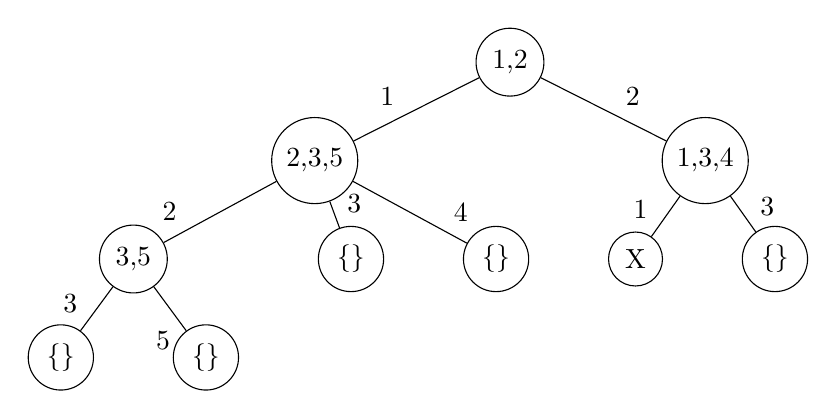
\begin{tikzpicture}[every tree node/.style={draw,circle},
   level distance=1.25cm,sibling distance=1cm,
   edge from parent path={(\tikzparentnode) -- (\tikzchildnode)}]
\Tree
[.1,2
    \edge node[auto=right,pos=.6] {$1$};
    [.2,3,5 
       \edge node[auto=right,pos=.8] {$2$};
       [.3,5 
       \edge node[auto=right,pos=.8] {$3$};
		  [.{$\{\}$} ]
	   \edge node[auto=right,pos=.8] {$5$};
	    	  [.{$\{\}$} ]    	
       	]
       \edge node[auto=left,pos=.8] {$3$};
       [.{$\{\}$} ]
       \edge node[auto=left,pos=.8] {$4$};
       [.{$\{\}$} ]
        ]
    \edge node[auto=left,pos=.6] {$2$};
    [.1,3,4
        \edge node[auto=right,pos=.8] {$1$};
        [.X ]
        \edge node[auto=left,pos=.8] {$3$};
        [.{$\{\}$} ]
        ]
]
\end{tikzpicture}
\caption{Early Termination trong HST Explanation \label{overflow}}
\end{figure}
Chúng ta bắt đầu di chuyển root node với tập $\{1,2\}$ là các phát biểu đầu tiên tìm được trong $O$ chứng minh được $O$ $\models$ $\alpha$, thực hiện tương tự các bước đã được miêu tả ở trên ta thu được node $\{3,5\}$ là các phát biểu giải thích cho $O$ $\models$ $\alpha$, tới lúc này ta có thể thấy tập chứ đường đi theo cạnh từ node $\{3,5\}$ tới root node là $P_{1}=\{2,1\}$. Nhìn về phía bên phải ta phát hiện khi mở rộng cạnh từ node $\{1,3,4\}$ ta thu được đường đi về root node là $P_{2}=\{1,2\}$, ta thấy $P_{1} \equiv P_{2}$ do vậy nên khi dán nhãn cho node kế tiếp (được đánh dâu \xmark cho \textit{closed} node) chúng ta sẽ bỏ $\{1,2\}$ khỏi $O$ để được $O^{'}=\{3,4,5\}$, sẽ có một node giống y như node $\{3,5\}$ sẽ xuất hiện lần nữa ở node kế tiếp này nên việc kết thúc ở đây là cần thiết vì chúng ta sẽ tiếp kiệm được việc kiểm tra lại $\{3,5\}$ như ở bên trái.
\paragraph{Justification Reuse} - Cách quan trọng thứ hai để tối ưu là sử dụng lại các kiểm chứng. Trong phiên bản không tối ưu sử dụng ở ví dụ ontology $\beta$ ở trên, kiểm chứng được tìm ra nhờ các giải thuật Blackbox hay Glassbox cho từng node $v$ được thêm vào cây. Kiểm chứng hay tập các phát biểu được sử dụng để dán nhãn $v$, được tính toán dựa trên $O \backslash S$, với $S$ là tập các nhãn trên đường đi từ $v$ về root node. Thay vì dùng Glassbox hay Blackbox để tính $J$ trong $O \backslash S$, chúng ta có thể làm theo cách sau: nếu HST chứa vài node khác $v^{'}$ mà được dán nhãn với kiểm chứng $J$, và $S$ không giao (có phần tử chung) với $J$ thì $J$ có thể được sử dụng làm nhãn cho $v$. Lý do là vì khi $J\subseteq$ $O$ và $S\cap J = \emptyset$ thì sẽ tồn tại trường hợp $J\subseteq O \backslash S$, từ đó $J$ được tính như một kiểm chứng cho để có thể dán nhãn $v$. Sử dụng lại các phát biểu chứng minh (hay kiểm chứng) sẽ giúp tiết kiệm nhiều lời gọi hàm không cần thiết tới Blackbox hoặc Glassbox từ đó tăng được hiệu năng.
\\
\paragraph{Kết luận} Trong quá trình nghiên cứu về các nguyên nhân gây inconsistency trong ontology, chúng em đã tìm hiểu được nhiều giải pháp đã được nghiên cứu và ứng dụng. Chúng em cũng nắm được nguyên lý hoạt động những giải thuật và quy trình này như HST Explaination ,Blackbox Algorithm \cite{axiomPinpoint}. Nguyên lý này được áp dụng trong các chứng năng giải thích của thư viện OWL-API \cite{owlapi}.



  % Giải pháp sửa chữa ontology


%% ----------------------------------------------------------------
% Now begin the Appendices, including them as separate files

\addtocontents{toc}{\vspace{2em}} % Add a gap in the Contents, for aesthetics

\appendix % Cue to tell LaTeX that the following 'chapters' are Appendices

%\input{Appendices/AppendixA}	% Appendix Title


\addtocontents{toc}{\vspace{2em}}  % Add a gap in the Contents, for aesthetics
\backmatter

%% ----------------------------------------------------------------
\label{Bibliography}
\lhead{\emph{Bibliography}}  % Change the left side page header to "Bibliography"
\bibliographystyle{IEEEtranN}  % Use the "unsrtnat" BibTeX style for formatting the Bibliography
\bibliography{Bibliography}  % The references (bibliography) information are stored in the file named "Bibliography.bib"

\end{document}  % The End
%% ----------------------------------------------------------------